
\documentclass{book}

\usepackage{lmodern}
\usepackage[T1]{fontenc}
\usepackage[spanish,activeacute]{babel}
\usepackage[utf8]{inputenc}
\usepackage{mathtools}
\usepackage{graphicx}
\usepackage{fancyhdr}
\usepackage{hyperref}
\usepackage{colortbl}
\usepackage[dvipsnames]{xcolor} 
\usepackage{enumerate} 
\usepackage{multirow}
%------------------Definimos los colores a usar----------------%
\definecolor{myWhite}{rgb}{250,250,250}
\definecolor{myBlue}{HTML}{166995}
\definecolor{myDarkBlue}{HTML}{0D547B}
\definecolor{myBlueRef}{HTML}{0277bd}
\definecolor{myBlueChapter}{HTML}{004784}


%---------Definimos el color de cada vínculo en el documento como links, urls, citas, etc.
\hypersetup{
    colorlinks=true,
    linkcolor=myBlue,
    filecolor=magenta,      
    urlcolor=myBlue,
    citecolor=myBlueRef,
    pdftitle={Sharelatex Example}
}

%--------------Define el tipo de numeración para la tabla de contendios---------------%

\frontmatter

%--------------Definimos el estilo del piede página------------------------------------%

\fancypagestyle{plain}{
  
  %\fancyfoot[LE]{\begin{picture}(0,0) \put(-165,-95){ 
\includegraphics[scale=1]{imagenes/foot.png}}\end{picture}}

  %-------------Imagen de pie de página pares---------%

    \fancyfoot[LE]{\begin{picture}(0,0) \put(-165,-95){ 
\includegraphics[scale=1]{imagenes/foot-azul.png}}\end{picture}}

  %-------------Imagen de pie de página impares---------%
    \fancyfoot[LO]{\begin{picture}(0,0) \put(-110,-95){ 
\includegraphics[scale=1]{imagenes/foot-azul.png}}\end{picture}}

  \renewcommand{\headrulewidth}{0.5pt}
  \renewcommand{\footrulewidth}{0.5pt}


}

\pagestyle{plain}% aplicamos el estilo para todas las páginas


%----------------Eliminamos la identación de los parrafos ------------% 
\setlength{\parindent}{0pt}

%-----------------Color para las cajas de texto de los capítulos-----------
\tcbset{colback=myBlueChapter!5!white,colframe=myBlueChapter!50!black, colbacktitle=myBlueChapter!80!black}






%-----------------------Comandos para los Casos de uso----------------------%
\newcommand{\actor}[0]{
\includegraphics[scale=.3]{imagenes/actor.png}  }%iucluye la imagen del actor
\newcommand{\sistema}[0]{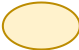
\includegraphics[scale=.3 ]{imagenes/system.png}  }%incluye la imagen del sistema
\newcommand{\finCU}[0]{\textit{- - - - Fin del caso de uso.}}
\newcommand{\finTA}[0]{\textit{- - - - Fin de la trayectoria.}}


%---------------------Comando para estilo de las reglas de negocio----------------%
\newcommand{\Dline}[2]{{\setlength{\parindent}{0pt}\textbf{\textcolor{myBlue}{\large{#1} \large{#2}}}} \\\rule[3mm]{110mm}{0.3mm}
\includegraphics[scale=.5]{imagenes/Documento.png}}%Linea de separadora 

\newcommand{\DGline}[2]{{\setlength{\parindent}{0pt}\textbf{\textcolor{myBlue}{\large{#1} \large{#2}}}} \\\rule[3mm]{110mm}{0.3mm}
\includegraphics[scale=.5]{imagenes/DocumentoG.png}}%Linea de separadora 

\newcommand{\DVline}[2]{{\setlength{\parindent}{0pt}\textbf{\textcolor{myBlue}{\large{#1} \large{#2}}}} \\\rule[3mm]{110mm}{0.3mm}
\includegraphics[scale=.5]{imagenes/DocumentoV.png}}%Linea de separadora 



%----------------Incluimos la sección de bibliografía a la tabla de contenidos--------%

\let\OLDthebibliography=\thebibliography
\def\thebibliography#1{\OLDthebibliography{#1}%
\addcontentsline{toc}{chapter}{\bibname}}



\begin{document}

    \begin{titlepage}

  \thispagestyle{empty}


  \begin{minipage}{.2\textwidth}
    \flushleft
%----------------imagenLineasGuia---------------------------%
    \center{
\includegraphics[scale=.19]{imagenes/ipn.pdf}}
    
    \vspace{20pt}

    \center{
      \rule{.5pt}{.6\textheight}
      \hspace{7pt}
      \rule{2pt}{.6\textheight}
      \hspace{7pt}
      \rule{.5pt}{.6\textheight}
    } 
  \end{minipage}
  \begin{minipage}{.8\textwidth}
  %---------------InfoTesis-------------------------%
    \flushright

    \center{

      \center{
        \LARGE{I}\large{NSTITUTO} \LARGE{P}\large{OLITÉCNICO} 
        \LARGE{N}\large{ACIONAL}
      } \\

      \rule{\textwidth}{1pt}\\
      \hrulefill\\[1cm]



      \LARGE{E}\large{SCUELA} \LARGE{S}\large{UPERIOR} \large{DE} \LARGE{C}\large{ÓMPUTO}\\[1cm]

      \large{ TRABAJO TERMINAL} \\[1cm]

      \textbf{ \LARGE{R}\LARGE{ecolector} \LARGE{y} \LARGE{clasificador} \LARGE{de}  
      \LARGE{noticias}}\\[1cm]
      \large{\textbf{2018-B013}}\\[1cm]


      \large{\textbf{PRESENTAN:}}\\[1cm]
      \large{CARLOS ANDRES HERNANDEZ GOMEZ}\\
      \large{LUÍS DANIEL MEZA MARTÍNEZ}\\[1cm]


      \large{\textbf{DIRECTORES:  }}\\[.5cm]
      \large{\textbf{M. en C.} JOEL OMAR JUÁREZ GAMBINO }\\
      \large{\textbf{Dra.} CONSUELO VARINIA GARCÍA MENDOZA }\\[0.5cm]

     \large{\textbf{CIUDAD DE MÉXICO}}\\
     \ \\
     \today

    }


  \end{minipage}
  \end{titlepage}

  
  
    \tableofcontents

  \mainmatter %Iniciamos la número ración del indice

  %-------------------------------Capitulos----------%

  
\chapter{Introducción}


\begin{Large}$\mathbf{E}$\end{Large}l artículo periodístico o noticia, es la información de un hecho de interés ocurrido en un periodo de tiempo determinado. Constituye el elemento primordial en la información de la prensa y del género básico del periodismo [1]. Conocer los acontecimientos del mundo independientemente del tema, día o lugar en el cual se han suscitado, tiene una gran importancia en la sociedad, se comparten por distintos medios de comunicación, tales como la televisión, redes sociales, diarios, blogs y la radio. Nos permiten conocer la situación económica del país, logros de la ciencia, desastres naturales, la situación en cuestión de inseguridad entre otros hechos. En el ámbito de las inversiones, crean expectativas y eso a su vez puede modificar los planes de inversión en cualquier sector, siendo así de suma importancia compartirlas de una forma eficaz [2].\\

El uso de páginas web como medio de comunicación está en incremento, permitiendo consultar noticias de distintos sitios como los periódicos electrónicos; su información al igual que un diario tradicional se encuentra dividida en secciones para facilitar la consulta, sin embargo, la clasificación suele variar en cada portal, incluso teniendo el mismo contenido. Un problema mayor se encuentra en los sitios independientes, los cuales no cuentan con una segmentación particular, haciendo difícil realizar una búsqueda eficaz.\\



\section{Problemática}


Los métodos tradicionales para la recopilación de información de los recolectores web (Crawler), están basados en las etiquetas o marcadores que los sitos añaden a su código fuente, por ejemplo, algunos artículos periodísticos son etiquetados a la sección que pertenecen (Política, deporte, cultura, etc). Sin embargo, existen muchas fuentes de información que no etiquetan sus publicaciones, incluso si la tarea es realizada, dicha segmentación no indica claramente el tipo de contenido; Al consultar los portales mas visitados en México (En el giro del periodismo) [3] se encuentra definida la sección deportes con varios sinónimos como \textbf{Universal deportes} (Diario \text{El universal}), \textbf{La afición} (\text{Milenio}), \textbf{Adrenalina} (\text{Excelsior}), etc. Como este ejemplo se encuentran mas. Las noticias son segmentadas de forma tan diversa que ha complicado su búsqueda en la Internet.\\


Para definir las etiquetas o marcadores con los cuales se clasifica la información de los sitios web, se requiere un proceso manual de análisis de la información. Este proceso implica tiempo y esfuerzo por parte de las personas que realizan el trabajo. Por lo anterior se plantea la necesidad de crear métodos para automatizar esta tarea. 

\section{Justificación}



Hoy en día existen distintas maneras de informarse acerca de los acontecimientos más recientes, por ejemplo, la televisión, blogs, redes sociales, foros,
diarios, etc. Esto ha provocado que la información se encuentre dispersa y
se deba acceder a múltiples recursos para ser recopilada, implicando
una inversión de tiempo y esfuerzo. Para facilitar esta tarea, existen herramientas
que hacen la búsqueda de noticias de interés para el usuario en forma automática. Sin embargo, dichas herramientas requieren que los sitios a consultar tengan etiquetas definidas y homogéneas.\\

Según el díario El Economista [3] el sitio web “Animal Político”
ocupa el lugar número cuatro en el ranking de medios nativos digitales, clasifica sus noticias de una manera poco habitual para los lectores como la sección
\textbf{El sabueso}, \textbf{El plumaje}, \textbf{Hablemos de . . . }, entre otras, lo que hace complicado obtener los artículos con los métodos tradicionales de recopilación que,
se basan sólo en las etiquetas que identifican cada sección y no el contenido de
las noticias.

%\lhead{ (www.animalpolitico.com)}
%\thispagestyle{ESTILO}

\section{Solución Propuesta}

Se propone crear una aplicación web el cual recolecte y clasifique noticias de acuerdo 
a su contenido y periodo de publicación. Finalmente, las noticias
que satisfagan ambos filtros (Tipo de contenido y fecha de publicación) serán mostradas al usuario.

\section{Objetivo}

  Crear un recolector de noticias, el cual permita recopilar información de diferentes fuentes como diarios, sitios de noticias, foros y mediante el análisis automático de su contenido muestre aquellas noticias que satisfagan los filtros establecidos por el usuario.
  

\section{Objetivos Específicos}
\begin{itemize}
  \item Desarrollar un recolector de noticias, el cual permita obtener información de diferentes fuentes como diarios, sitios de noticias, blogs y foros
  \item Analizar de forma automática el contenido de las noticias para satisfacer los filtros establecidos por el usuario
  \item Mostrar el enlace (URL) de las noticias que cumplieron con los filtros establecidos
  \item Afinar el clasificador de noticias realizado en el trabajo terminal 2017-A02 para utilizarlo en el contexto de esta propuesta (filtro de sección) 

\end{itemize}
  \newpage
  
\chapter{Estado del arte}\label{chp:EstadoArte}

\section{Introducción}

	A continuación, se mostrarán distintos trabajos nacionales e internacionales, así como herramientas las cuales desempeñan una labor similar al propuesto en este trabajo.\\

\section{Trabajos nacionales}%[pdf]

	El trabajo \textit{Clasificación Automática de Textos de Desastres Naturales en México}
	propone clasificar noticias del ámbito en Desastres Naturales, utilizando estrategias de reducción de dimensionalidad conocidas como umbral en la frecuencia y ganancia en la información, los métodos de clasificación utilizados fueron el clasificador simple de Bayes y vecinos más cercanos.\\

	Se utilizaron 375 noticias del periódico \"Reforma\" como conjunto de entrenamiento, para posteriormente clasificarlas (relevantes e irrelevantes), de los cuales el 11.5\% de noticias eran relevantes y el 88.5\% restante eran irrelevantes.\\

	Una vez obtenido el conjunto de noticias se procedió con un pre\-procesamiento, el cual reducía el tamaño de los documentos, eliminando las partes de los textos que no se consideraban relevantes; posteriormente se realizó el indexado, el cual los documentos son representdos por vectores de palabras en un espacio de dimensionalidad \textit{n} en el cual se logró una reducción de dimensionalidad en donde finalemente se utilizaron técnicas de clasificación como el algoritmo simple de Bayes en el cual se obtuvo un resultado del 97\% de efectividad al clasifciar noticias de desastres naturales.\\



\section{Trabajos internacionales}
	%https://scielo.conicyt.cl/scielo.php?script=sci_arttext&pid=S0718-09342014000300001
	La obra \textit{Clasificación Automática de Textos Usando Redes de Palabras} propone un algoritmo para la clasificación automática de textos basado en una representación y clasificación distinta utilizada en los algoritmos de clasificación supervisada, utilizando redes de palabras.\\

	Se utilizaron 1000 mensajes de texto de la plataforma Twitter, en el idioma español y correspondiente a distintos contextos, para posteriormente clasificar el tipo de contenido de los mensajes (positivos, negativos y neutrales), se definió un grafo como aquella red de palabras co\-cocurrentes construida a partir de un conjunto de textos clasificados; para su realización el primer proceso es llevar distintas variantes de una misma palabra a su raíz, esto para reducir la variabilidad del lenguaje posteriormente se considera las palabras plurales (terminadas con ‘s’ o ‘es’). A estas se les elimina el sufijo para compararlas con su equivalente singular, realizando el cambio de manera automática.
	Los resultados mostraron que el clasificador presenta un 80\% cercanía respecto a la clasificación realizada por una persona; su nivel de desempeño fue mayor al obtenido con el algoritmo Naive Bayes.\\


	El trabajo \textit{Document Classification for Newspaper Articles} se ha enfocado en clasificar articulos del MIT (Massachusetts Institute of Technology) de las siguientes categorías:

	\begin{itemize}
		\item Arts
		\item Features
		\item News
		\item Opinion
		\item Sports
		\item World
	\end{itemize}

	Para los cuales utilizarón el algoritmos de clasificación como el \textit{Naive Bayes} ya que era uno de los clasificadores más simples y eficaces que otras técnicas de clasificación, de igual manera utilizarón la clasificación máxima de entropia el cual provee segmentación de texto, modelado de lenguaje.
	Se utilizó un corpus de 3000 artículos en total, siendo 500 artículos de cada sección mencionada. Para el entrenamiento se utilizaron 120 artículos siendo 20 de cada sección y teniendo como resultado un 77\% de exactitud.\\

\section{Herramientas disponibles}

	Entre las herramientas utilizadas para el procesamiento de lenguaje natural y aprendizaje automático se encuentran:

	%https://cloud.google.com/natural-language/?hl=Es-419
	\begin{itemize}
		\item \textit{Google Cloud Natural Language}; Ha revelado la estructura y el significado del texto con modelos potentes de aprendizaje automático previamente entrenados en una API de REST fácil de usar y con modelos personalizados se puede utilizar para extraer información sobre personas, lugares, eventos y muchos otros datos, que se mencionan en documentos de texto, artículos periodísticos o entradas de blog. También se puede utilizar para comprender las opiniones sobre sus productos expresadas en los medios sociales o analizar la intención en las conversaciones de los clientes que se den en un centro de atención telefónica o una aplicación de mensajería[]
		\item Algoritmo Naive Bayes
		\item Procesamiento de lenguaje natural
		\item Árbol de decisión
		\item Clasificación máxima de entropía
	\end{itemize}

  \newpage
  
\Tlabel{CP1}\TChapter{Marco teórico}{gama}
\ \\\\
%---------------------------------Introducción--------------------------------%
En este capítulo se expondrán de manera detallada y ordenada el conjunto de conocimientos que permitirán comprender y analizar el tema propuesto. \\

La Figura \ref{fig:MarcoT} muestra los campos abarcados por la investigación.
A continuación cada área sera desarrollada con los conceptos de interés para la solución propuesta.

\begin{figure}[H]
	\centering
	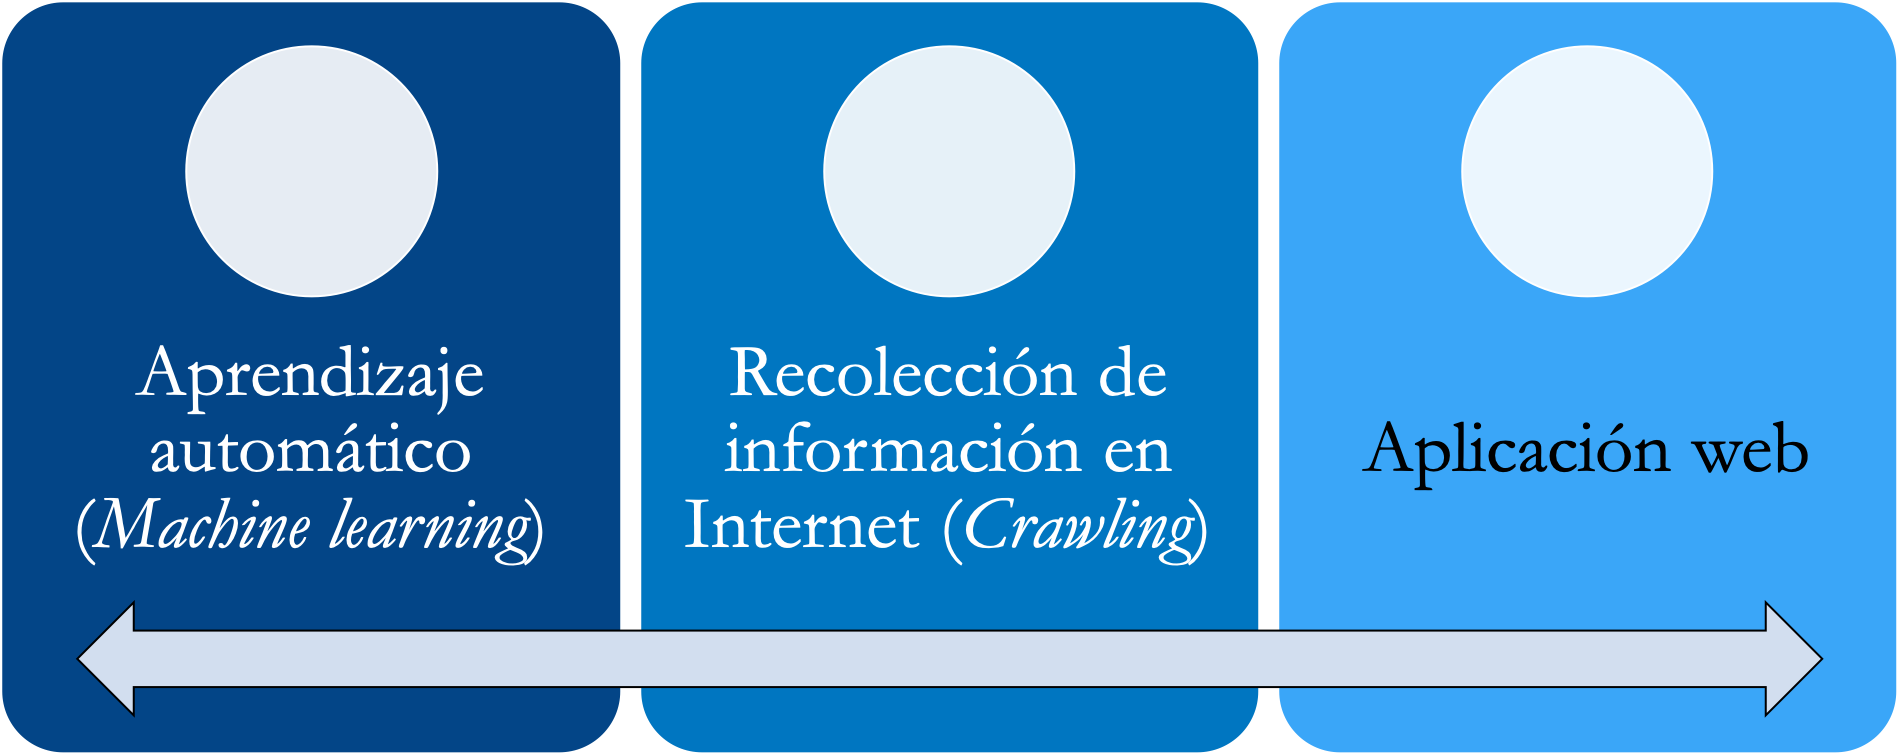
\includegraphics[scale=.35]{imagenes/Capitulo3/Marco.png}
	\caption{Campo de estudio}
	\label{fig:MarcoT}
\end{figure}

%---------------------------------Conceptos-------------------------------------%
%Recordar renombrar las citas




%------------------------------------Inteligencia Artificial-------------------------------%
\section{Inteligencia Artificial}

Son muchas las definiciones que se encuentran de la inteligencia artificial o IA, en sus inicios se propone como las  actividades asociadas al pensamiento humano, tareas como, toma de decisiones, resolución de problemas y aprendizaje \citep{CT19}.


Con el paso de los años se ha acuñado una definición mas completa: `la Inteligencia Artificial es una ciencia orientada al diseño y construcción de máquinas que implementen tareas propias de humanos dotados de inteligencia'' \citep{CT1}.\\


Esta ciencia contribuye en el desarrollo de diversos campos de investigación como, Redes neuronales, Computación evolutiva, Algoritmos genéticos, Programación Genética, Teoría del caos. Además tiene un campo amplio de aplicaciones en la sociedad \citep{CT20}, a continuación se muestran algunos ejemplos:

\begin{itemize}
	\item \textbf{Vehículos robóticos}: Un auto robótico sin conductor llamado STANLEY aceleró a través del terreno de Mojave a 22 mph, terminando el curso de 132 millas primero para ganar el Gran Desafío DARPA 2005.

	\item \textbf{Reconocimiento de voz}: Un viajero que llama a \textit{United Airlines} para reservar un vuelo puede tener la conversación completa guiada por un sistema automático de reconocimiento de voz y gestión de diálogos.

	\item \textbf{Planificación y programación autónoma}: A cien millones de millas de la Tierra, el programa \textit{Remote Agent} de la NASA se convirtió en el primer programa autónomo de planificación a bordo para controlar la programación de operaciones de una nave espacial.

	\item \textbf{Robótica}: \textit{iRobot Corporation} ha vendido más de dos millones de aspiradoras robóticas \textit{Roomba} para uso doméstico.

	\item \textbf{Máquina traductora}: Un programa de computadora  traduce automáticamente del árabe al inglés.

\end{itemize} 

%------------------------------------Apredizje automático-------------------------------%
\section{Aprendizaje Automático}

EL Aprendizaje Automático es una rama de la Inteligencia Artificial, permite  desarrollar algoritmos que tienen la capacidad de predecir
continuamente los cambios que se puedan suscitar en un problema específico\citep{CT2}.\\

EL campo utiliza una variedad de algoritmos que aprenden iterativamente de datos para mejorar, describir 
datos y predecir resusltados. A medida en la cual los algoritmos de entrenamiento obtienen datos es posible obtener 
modelos más precisos basados en esos datos. Un modelo de Aprendizaje Automático es una salida generada cuando se tiene 
entrenado un algoritmo de Aprendizaje Automático. Después de entrenar el modelo con una entrada de datos, obtendremos 
una salida. Por ejemplo, un algoritmo predictivo creará un modelo predictivo. Luego, cuando se le proporciona datos 
al modelo predictivo, se obtendrá una predicción basada en los datos que entrenaron al modelo .
\\
%https://www.ibm.com/downloads/cas/GB8ZMQZ3
%Aprendizaje Automático es un método de análisis de datos el cual permite automatizar la obtención de 
%resultados a partir de una numerosa cantidad de datos. Es una disciplina de la Inteligencia 
%Artificial la cual permite optimizar operaciones, realizar predicciones basadas en la información 
%que se le proporcione.
\\
Algunas de las áreas en las cuales Aprendizaje Automático se ha visto involucrada es \citep{CT3}:
\begin{itemize}
	\item Servicios financieros: Las empresas pueden detectar insights en la información de sus clientes 
	y sus operaciones, permitiendo de manera automatizada la recomendacion de productos financieros al usuario 
	indicado y en el momento preciso.
	\item Salud: En combinación con sensores o dispositivos en prendas de vestir (weareble devices) 
	un sistema puede monitorear y valorar el estado de salud de una persona en tiempo real, y si detecta 
	una irregularidad, tomar una acción en forma automática.
	\item Ventas y mercadotecnia: A partir de compras previas por el usuario se pueden realizar 
	realizar recomendaciones con alto potencial de éxito. Este conocimiento del cliente también ayuda a implementar 
	campañas de marketing con gran nivel de precisión.
	\item Gobierno:  El gobierno puede analizar su gigantesco cúmulo de datos, y detectar ágilmente áreas o
	funciones cuya mejora debe ser prioritaria –de esta forma, los recursos	públicos se invierten en los ámbitos 
	correctos, aquellos que realmente mejoran la vida de la ciudadanía y evitan procesos lentos y burocráticos.
	\item Transporte: Las compañías analizan sus operaciones de negocio y rápidamente detectan rutas más
	eficaces, lo que incrementa la rentabilidad de sus procesos (tiempos de entrega más cortos, con menor consumo 
	de combustible, menor riesgo de desperfectos y menor desgaste de las unidades).
\end{itemize}

\subsection{Aprendizaje supervisado}
Los algoritmos de aprendizaje supervisado dependen de datos previamente etiquetados, es decir necesita de un entrenamiento para 
que el algoritmo pueda comprender los datos y con ello determinar que etiqueta debe asignarse a los nuevos datos 
en función del patron y asociando los patrones a los nuevos datos sin etiquetar. Después de ello, la maquina recibe 
un nuevo conjunto de datos para que el algoritmo de aprendizaje supervisado analice los datos y produzca un resultado 
correcto de los datos etiquetados \citep{CT4}.

\subsubsection{Regresión líneal}
La regresión es una técnica estadística utilizada para estudiar la relación entre dos variables, permite hallar el valor esperado de 
una variable aleatoria a cuando b toma un valor específico. La aplicación de este método implica un supuesto de linealidad cuando 
la demanda presenta un comportamiento creciente o decreciente, por tal razón, se hace indispensable que previo a la selección de 
este método exista un análisis de regresión que determine la intensidad de las relaciones entre las variables que componen el modelo.
\\
El pronóstico de regresión lineal simple es un modelo óptimo para patrones de demanda con tendencia (creciente o decreciente), 
es decir, patrones que presenten una relación de linealidad entre la demanda y el tiempo \citep{CT5}.

La Figura \textbf{\ref{fig:RL}} muestra un ejemplo de los resultados obtenidos utilizando regresión líneal. 

\begin{figure}[H]
  \centering
  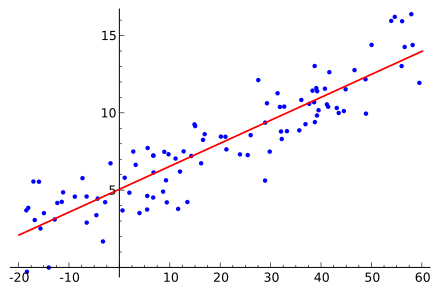
\includegraphics[scale=.6]{imagenes/Capitulo3/regresionLineal}
  \caption{Regresión lineal con una variable dependiente y una variable independiente.}
  \label{fig:RL}
\end{figure}
%https://cleverdata.io/conceptos-basicos-machine-learning/

\subsubsection{Regresión logística}
La regresión logística es una técnica estadística multivariante que nos permite estimar la relación existente entre una variable dependiente 
no métrica (donde la variable es binaria o también conocida como dicotómica, es decir, solo va a dar como resultado dos alternativas posibles) 
y un conjunto de variables intependientes métricas o no métricas \citep{CT6}. Es útil para modelar la probabilidad de un evento ocurriendo como 
función de otros factores. El análisis de regresión logística se enmarca en el conjunto de Modelos Lineales Generalizados que usa como función de 
enlace la función logit. Las probabilidades que describen el posible resultado de un único ensayo se modelan, como una función de variables explicativas, 
utilizando una función logística.

La regresión logística es usada extensamente en las ciencias médicas y sociales. Otros nombres para regresión logística usados en varias áreas de 
aplicación incluyen modelo logístico, modelo logit, y clasificador de máxima entropía.


\subsubsection{Na{\"i}ve bayes}
Na{\"i}ve Bayes es un conjunto de algoritmos de aprendizaje supervisado que se basan en la aplicación del teorema de Bayes con "Na{\"i}ve" 
(Ingenuo) la cual es la supuesta de independencia condicional entre cada par de características dado el valor de la variable de clase. 

La clasificación Naive Bayes son aproximaciones probabilísticas, las cuales hacen especulaciones sobre como deben de ser 
generados los datos. Generalmente utilizan aprendizaje supervisado sobre el conjunto de entrenamiento para poder esimar los parámetros 
del modelo generativo, en tanto el conjunto de datos de entrada nuevos se realiza el teorema de Bayes, seleccionando la probable categoría 
que se ha generado \cite{CT7}.
\\
Todas las características extraídas que utilizan este clasificador son independientes entre sí. La ventaja de usar este clasificador es que 
funciona bien tanto con datos numéricos como con datos textuales y, además, es más fácil de implementar. La desventaja de este clasificador es 
que su rendimiento empeora cuando las características extraídas se correlacionan entre sí.

\subsubsection{Maquina de soporte vectorial}
Las maquinas de soporte vectorial son un conjunto de algoritmos de aprendizaje los cuales se basan en el uso de un espacio de funciones lineales, 
el cual se encuentra con mas dimensiones inducido por un kernel, en el que las hipotesis son las entradas para el algoritmo. \\
El algoritmo induce separadores lineales ya sea en el espacio original de los ejemplos de entrada, si los datos no son separabales se busca un hiperplano 
en el que si lo sean, se hace de forna implicita con las funciones kernel.\\

Estos métodos están propiamente relacionados con problemas de clasificación y regresión. Dado un conjunto de ejemplos de entrenamiento (de muestras) 
podemos etiquetar las clases y entrenar una SVM para construir un modelo que prediga la clase de una nueva muestra. Intuitivamente, una SVM es un modelo 
que representa a los puntos de muestra en el espacio, separando las clases a 2 espacios lo más amplios posibles mediante un hiperplano de separación definido 
como el vector entre los 2 puntos, de las 2 clases, más cercanos al que se llama vector soporte. Cuando las nuevas muestras se ponen en correspondencia con dicho 
modelo, en función de los espacios a los que pertenezcan, pueden ser clasificadas a una o la otra clase \citep{CT8}.

\subsubsection{Random forest}
Random forest es una combinación de árboles predictiroes, de modo que cada árbol depende de los valores de un vector 
aleatorio muestreado independientemente y con la misma distribución para cada uno de estos. Es una modificación sustancial de bagging que construye una 
larga colección de árboles no correlacionados y posteriormente los promedia \citep{CT9}.

\subsection{Aprendizaje no supervisado}
Los algoritmos de aprendizaje no supervisado no dependen de datos previamente etiquetados, por lo cual los algoritmos 
tienen la tarea de agrupar la información no clasificada según sus similitudes, patrones y diferencias sin ningún entrenamiento 
previó de datos, por lo cual aprenden gracias a la cantidad de datos que le son ingresadas con características propias de un 
objeto y con ello pueda determinar los resultados basados en los datos de entrada \citep{CT10}.
%https://towardsdatascience.com/supervised-machine-learning-classification-5e685fe18a6d

\section{Procesamiento de lenguaje natural}
El procesamiento de lenguaje natural es una disciplina de la Inteligencia Artificial que se ocupa de la formulación e 
investigación de mecanismos computacionales para la comunicación entre personas y maquinas mediante el uso de Lenguajes 
Naturales.

El procesamiento del lenguaje natural incluye diferentes técnicas para interpretar el lenguaje humano, que van desde los métodos 
estadísticos y del aprendizaje basado en máquina hasta los enfoques basados en reglas y algorítmicos. Necesitamos una amplia variedad 
de métodos porque los datos basados en texto y en voz varían ampliamente, al igual que las aplicaciones prácticas. 

Las tareas básicas de NLP incluyen la simbolización y el análisis sintáctico , lematización/derivación, etiquetado de la parte del 
habla, detección del lenguaje e identificación de relaciones semánticas. Si alguna vez creó diagramas de enunciados en la primaria, 
ya ha realizado estas tareas de forma manual antes. 

En términos generales, las tareas NLP dividen el lenguaje en piezas elementales más cortas, intentan entender las relaciones entre 
las piezas y exploran cómo funcionan las piezas juntas para crear significado \citep{CT11}.

Estas tareas implícitas se utilizan a menudo en recursos NLP de más alto nivel, como:
\begin{itemize}
	\item Categorización de contenido. Un resumen del documento basado en la lingüística, 
	incluyendo búsqueda e indización, alertas de contenido y detección de duplicación.
	\item Descubrimiento y modelado de temas. Capture con precisión el significado y temas en colecciones de texto, y 
	aplique analítica avanzada a texto, como optimización y pronósticos.
	\item Extracción contextual. Extraiga automáticamente información estructurada de fuentes basadas en texto.
	\item Análisis de sentimiento. Identificación del estado de ánimo u opiniones subjetivas en grandes cantidades de 
	texto, incluyendo minería de sentimiento y opiniones promedio. 
	\item Conversión de habla a texto y de texto a habla. Transformación de comandos de voz en texto escrito y viceversa. 
	\item Sumarización de documentos. Generación automática de sinopsis de grandes cuerpos de texto.
	\item Traducción basada en máquina. Traducción automática de texto o habla de un idioma a otro.
\end{itemize}

%\subsection{Lenguaje}
%El lenguaje es un medio de comunicación a traves de de un sistema de símbolos \cite{dieciseis}.
%La Real Academía Española define al lenguaje como la facultad del ser humano de expresarse y comunicarse con los demás 
%a través del sonido articulado o de otros sistemas de signos.

\subsection{Tokenización}
Es el proceso que descompone los textos de una colección en sus unidades mínimas, las palabras
o términos propiamente dichos. A tales elementos se les denomina tokens que conforman una lista de
ítems que se utiliza para su análisis estadístico, ling{\"u}ístico, de almacenamiento y posteriormente de
recuperación de información. Los tokens a su vez pueden ser identificados mediante una codificación
ASCII o en su defecto hexadecimal, con el objeto de facilitar la identificación uno a uno cada caracter
que compone la palabra. De hecho, este proceso permite la identificación de cadenas de caracteres de
forma unívoca, de cara a posteriores tratamientos de depuración, eliminación de signos de puntiación
o la reducción morfológica \citep{CT12}.

Ejemplo  (\ref{tabla:sencilla}): Hoy es un gran día para salir.

\begin{table}[htbp]
	\begin{center}
	\begin{tabular}{|lrrccccc|}
		\hline
		ID & 1 & 2 & 3 & 4 & 5 & 6 & 7 \\ 
		Token & Hoy & es & un & gran & día & para & salir \\ \hline
		\hline
	\end{tabular}
	\caption{Ejemplo de tokenización}
	\label{tabla:sencilla}
	\end{center}
	
\end{table}


\subsection{Lematización}
Es el proceso lingüstico que, dada una palabra flexionada se encuentra su
lema. Una palabra flexionada es cuando esta en el plural, en femenino conjugada,
diminutivo o en superlativo. El lema es la palabra que esta en singular para
sustantivo, singular masculino para adjetivo e infinitivo para un verbo \citep{CT13}. Ejemplo:

	\begin{itemize}
		\item amigos, amiga, amiguitos-> Amigo
		\item soy, son, es->Ser
	\end{itemize}

Cabe mencionar que existen diversos grados de lematización

	\begin{itemize}
		\item Mórfólogica: Es la anterior mente explicada
		\item Sintáctica: Toma encuenta el contexto donde se encuentra la palabra

	\end{itemize}

Una opción para lematizar es Freeling \citep{CT18}, este es un lematizador hecho por la
universidad de catalunia.

\section[Representación del t.]{Representación del texto}
Los métodos de Aprendizaje Automático requieren que la información de la cual aprenderán esté representada en un
formato que facilite su procesamiento. Generalmente esta representación es mediante vectores de valores numéricos. 
Cuando se requiere utilizar estos métodos con información en forma de texto, dicha
información debe ser transformada para generar una representación más adecuada. 

\section{Corpus}
Se le llama corpus a la recopilación de un conjunto de textos, de materiales escritos y/o hablados, 
agrupados bajo un conjunto de criterios mínimos, para realizar ciertos análisis lingüísticos.


\section{Crawler}
Un crawler \citep{CT14} es una herramienta la cual analiza sitios web, permitiendo recolectar 
las páginas web para así posteriormente extraer la información que contengan. Un crawler también 
conocido como como robot o spider, es un sistema para la descarga masiva de páginas web. Son uno de 
los componentes principales de los motores de búsqueda web, los sistemas que reúnen un conjunto de 
páginas web, las indexan y permiten a los usuarios realizar consultas contra el índice y encontrar las 
páginas web que coincidan con las consultas.


\section{Sitios web}
Un sitio web \citep{CT15} es un conjunto de páginas web interconectadas y de acceso público que comparten 
un solo nombre de dominio. Los sitios web pueden ser creados y mantenidos por un individuo, grupo, empresa 
u organización para cumplir una variedad de propósitos. Todos estos sitios constituyen la World Wide Web. 

\subsection{Página web}
Una página web es un documento electrónico el cual forma parte de la WWW (\textit{World Wide Web}) generalmente 
construido en el lenguaje HTML (\textit{Hyper Text Markup Language}). Este documento puede contener enlaces que nos 
direcciona a otra página web. Para visualizar una página web es necesario de un browser o un navegador \citep{CT16}. 
Dentro de las páginas web podemos encontrar un sinfin de sitios los cuales pueden ser de nuestro interés.

\subsection{Blog}
Un blog es una página web en la cual el usuario no necesita conocimientos específicos del medio electrónico ni del 
formato digital para poder aportar contenidos de forma inmediata, ágil y constante desde cualquier punto de conexión 
a Internet \citep{CT17}. En un blog el usuario puede compartir cualquier tipo de información que sea de su agrado, 
teniendo una mayor libertad de expresión lo cual permite que otras personas compartan y comenten su manera de expresarse.

\subsection{Foro}
Un foro es una herramienta de comunicación asíncrona. Los foros permiten la comunicación de los participantes desde 
cualquier lugar en el que  esté  disponible  una  conexión  a Internet  sin  que  éstos  tengan  que  estar dentro del 
sistema al mismo tiempo, de ahí su naturaleza asíncrona. Brindando una mayor interacción entre distintos 
participantes y permitiendo conocer la opinión sobre un tema de distintas personas.



  \newpage
  \chapter{Análisis y diseño}

En este capítulo se describe el análisis y el diseño del trabajo propuesto para
la recolección, clasificación de noticias y el entorno web.

%------------------------Requisitos Funcionales ------------------%
\section{Requisitos funcionales}

%----------------------------RF1------------------------------%
   \Dline{RF1}{Recolectar noticias}
    \begin{itemize}
      \item \textbf{Descripción:} El sistema debe recolectar noticias de forma automática en Internet.\\
    \end{itemize}
%----------------------------RF2------------------------------%
   \Dline{RF2}{Clasificar noticias}
    \begin{itemize}
      \item \textbf{Descripción:} El sistema debe clasificar las noticias recolectadas de acuerdo a su contenido.\\
    \end{itemize}
%----------------------------RF3------------------------------%
   \Dline{RF3}{Mostrar resultados}
    \begin{itemize}
      \item \textbf{Descripción:} El sistema mostrará las URLs de las noticias que cumplan con los criterios de búsqueda establecidos.\\
    \end{itemize}


%------------------------Requisitos No Funcionales ---------------%
\section{Requisitos no funcionales}



%----------------------------RNF1------------------------------%
   \DVline{RNF1}{Tiempo de clasificación}
    \begin{itemize}
      \item \textbf{Descripción:} La clasificación de una noticia no debe tardar mas de cinco segundo.\\
    \end{itemize}

%----------------------------RNF2------------------------------%
   \DVline{RNF2}{Número de palabras}
    \begin{itemize}
     \item \textbf{Descripción:} Las noticias recolectads deberán tener un mínimo de 180 palabras en ellas.\\
    \end{itemize}

%----------------------------RNF3------------------------------%  
   \DVline{RNF3}{Número de noticias mostradas}
    \begin{itemize}
      \item \textbf{Descripción:} En el sitio web, se den visualizar almenos 15 noticias.\\
    \end{itemize}

%----------------------------RNF4------------------------------%  
   \DVline{RNF4}{Tiempo de actualización}
    \begin{itemize}
      \item \textbf{Descripción:} El tiempo para mostrar las 15 noticias clasificadas no debe exceder los 3 segundos.\\
    \end{itemize}


%----------------------------Reglas de negocio---------------------%  
\section{Reglas de negocio}


En esta sección se describen las reglas de negocio implementadas en el trabajo propuesto.\\\\
%------------------RN1-----------------------%
\DGline{RN1}{Número de palabras}
\begin{itemize}
  \item \textbf{Tipo:}  
  \item \textbf{Descripción:}  La notica debe tener almenos 180 palabras
  \item \textbf{Ejemplo:}
  \item \textbf{Refer:}
\end{itemize}
%------------------RN2-----------------------%
\DGline{RN2}{Lenguaje de direcciones web}

\begin{itemize}
  \item \textbf{Tipo:}  
  \item \textbf{Descripción:} Las direcciones de los sitios a consultar deben estar redactadas en lenguaje español.
  \item \textbf{Referenciado por:} \Tref{CU1}{CU1 Seleccionar sección} \\
\end{itemize}
%------------------RN3-----------------------%
\DGline{RN3}{Lenguaje de noticias}

\begin{itemize}
  \item \textbf{Tipo:}  
  \item \textbf{Descripción:} Las noticias deben estar redactadas en lenguaje español mexicano.
  \item \textbf{Ejemplo:}
  \item \textbf{Referenciado por:}  \\
\end{itemize}
%------------------RN4-----------------------%
\DGline{RN4}{Restricción en la recoleción}

\begin{itemize}
  \item \textbf{Tipo:}  
  \item \textbf{Descripción:} Solo se puede recoletar información de los sitios que lo permitan.
  \item \textbf{Ejemplo:}
  \item \textbf{Referenciado por:}  \\
\end{itemize}
%------------------RN5-----------------------%
\DGline{RN5}{Porcentaje de aceptación}

\begin{itemize}
  \item \textbf{Tipo:}  
  \item \textbf{Descripción:} Solo se puede mostrar una noticia si cumple con un porcentaje de aceptación mayor a 60\%.
  \item \textbf{Ejemplo:}
  \item \textbf{Referenciado por:}  \\
\end{itemize}
%------------------RN6-----------------------%
\DGline{RN6}{Formato de fecha}

\begin{itemize}
  \item \textbf{Tipo:} Derivación.
  \item \textbf{Descripción:} El formato de fecha se define como:\\

  $F=D/M/A$

  $donde$\\ 

  $D=\{x/x\ E\ N,1\leq\ x\ \leq31\}$\\
  $M=\{y/y\ E\ N,1\leq\ y\ \leq12\}$\\
  $A=\{z/z\ E\ N,1990\leq\ z\ \leq\Lambda_i\}$\\

  $F:Fecha$\\
  $\Lambda_i:Anio\_actual$\\

  \item \textbf{Ejemplo:} 
  \item \textbf{Referenciado por:} \Tref{CU2}{CU2 Buscar noticias} \\
\end{itemize}

%------------------RN7-----------------------%
\DGline{RN7}{Perido preestablecido}

\begin{itemize}
  \item \textbf{Tipo:} Cálculo
  \item \textbf{Descripción:} El formato de fecha es el descrito en la \RNref{RN6}{Formato de fecha}; El periodo preestablecido se define de la siguiente forma.\\\\
  \textbf{Fecha fin}:Toma el valor de la fecha actual.\\
  \textbf{Fecha inicio}: Es colocada 5 día antes de la fecha actual; Se muestra la forma completa para el cálculo del día, mes y año:\\
  $Sea$\\
  $D_a:Dia\_actual$\\
  $M_a:Mes\_actual$\\
  $A_a:Anio\_actual$\\
  $F_i:Fecha\_inicio$\\
  $mod:Operacion\ modulo$\\
  $\Psi(M_a):Funcion\ dias\ de \ mes$\\

  $\xi=\frac{D_a-5}{\mid D_a-5 \mid}$\\

  $\delta=\frac{\xi(\mid\xi-1\mid)}{2}$\\

  La fecha toma el sigueinte valor:\\
  $F_i=D_c/M_c/A_c$\\ 
  Existen 4 casos para calcular el día, mes y años; Dependen del mes y el día actual: \\

  \begin{tabular}{|l|c|c|}
  	\hline
	\multicolumn{1}{| >{\columncolor{black}}l|}{ \textcolor{myWhite}{\textbf{Caso:}} }&
	\multicolumn{1}{| >{\columncolor{black}}c|}{ \textcolor{myWhite}{1} }&\multicolumn{1}{| >{\columncolor{black}}c|}{ \textcolor{myWhite}{2} }\\
	\hline
	\textbf{Restricción:}&$2\leq\ M_a\leq\ 12;D_a\neq5$  &$2\leq\ M_a\leq\ 12;D_a=5$\\
	\hline 
	\textbf{$D_c:$}&$(D_a-5)\pmod{\Psi(M_a-1)+1}$   &$\Psi(M_a-1)$\\
	\hline
	\textbf{$M_c:$}&$M_a+\delta$        			 &$M_a-1$\\
	\hline
	\textbf{$A_c:$}&$A_a$        				     &$A_a$\\
	\hline
  \end{tabular}


  \begin{tabular}{|l|c|c|}
  	\hline
	\multicolumn{1}{| >{\columncolor{black}}l|}{ \textcolor{myWhite}{\textbf{Caso:}} }&
	\multicolumn{1}{| >{\columncolor{black}}c|}{ \textcolor{myWhite}{3} }&\multicolumn{1}{| >{\columncolor{black}}c|}{ \textcolor{myWhite}{4} }\\
	\hline
	\textbf{Restricción:}&$M_a=1;D_a \neq 5$&\ \ \ \ \ \ $M_a=1;D_a=5$\ \ \ \ \ \\
	\hline 
	\textbf{$D_c:$}&\ \ \ \ \ \ \ \ \ $(D_a-5)\pmod{32}$\ \ \ \ \ \ \ \ & $31$\\
	\hline
	\textbf{$M_c:$}&$\xi\pmod{13}$&$12$\\
	\hline
	\textbf{$A_c:$}&$A_a+\delta$&$A_a-1$\\
	\hline
  \end{tabular}


  \item \textbf{Ejemplo:} 
  \item \textbf{Referenciado por:} \Tref{CU1}{CU1 Seleccionar sección}, \Tref{CU2}{CU2 Buscar noticias} \\
\end{itemize}%------------------RN8-----------------------%
\DGline{RN8}{Periodo válido}

\begin{itemize}
  \item \textbf{Tipo:} Derivación.
  \item \textbf{Descripción:}\\
  $Sea$\\

  $F_i:Fecha\_inicio$\\
  $F_f:Fecha\_fin$\\

  $T=\{Valido,Invalido\}$\\
  $\psi\ \epsilon\ T$\\

  Un periodo de fecha se defino como:\\

  $(\psi=Valido)\leftrightarrow(F_i\ \leq\ F_f)$\\
  $(\psi=Invalido)\leftrightarrow(F_i\ >\ F_f)$\\
  \item \textbf{Ejemplo:}
  \item \textbf{Referenciado por:} \Tref{CU2}{CU2 Buscar noticias} \\
\end{itemize}
%------------------RN9-----------------------%
\DGline{RN9}{Límite de periodo}

\begin{itemize}
  \item \textbf{Tipo:} Derivación. 
  \item \textbf{Descripción:} 

  $Sea$\\

  $F_i:Fecha\_inicio$\\
  $F_f:Fecha\_fin$\\
  $F_a:Fecha\_actual$\\
  $F_c:01/01/1990$\\

  $T=\{Valido,Invalido\}$\\
  $\psi\ \epsilon\ T$\\

  $\Phi=[F_c,F_a]$\\
  $I=[F_i,F_f]$\\
  

  Un intervalo de tiempo dentro de los limites del sistema se define como:\\

  $(\psi=Valido)\leftrightarrow(I\ \subseteq\ \Phi)$\\
  $(\psi=Invalido)\leftrightarrow(I\ \nsubseteq \Phi)$\\

  \item \textbf{Referenciado por:} \Tref{CU2}{CU2 Buscar noticias} \\
\end{itemize}

%------------------RN10-----------------------%
\DGline{RN10}{Campos obligatorios}

\begin{itemize}
  \item \textbf{Tipo:} Restricción.  
  \item \textbf{Descripción:} Los campos marcados con \* no se deben omitir.
  \item \textbf{Ejemplo:} 
  \item \textbf{Referenciado por:}  \\
\end{itemize}
%------------------RN11-----------------------%
\DGline{RN11}{Sitios restringidos}

\begin{itemize}
  \item \textbf{Tipo:}m
  \item \textbf{Descripción:} No se debe acceder a las siguientes páginas:
    \begin{itemize}
        \item Facebook
        \item Youtube
        \item Twitter
        \item Instagram 
    \end{itemize} 
  \item \textbf{Ejemplo:}
  \item \textbf{Referenciado por:} \Tref{CU3}{CU3 Recolectar noticias} \\
\end{itemize}
%------------------RN12-----------------------%
\DGline{RN12}{Orden de publicación}

\begin{itemize}
  \item \textbf{Tipo:} Descripción
  \item \textbf{Descripción:} Las noticias se muestrán de forma descendente deacuerdo a su fecha de difusión; Es decir la primera publicación en mostrarse es aquella que tiene la fecha y hora mas sercana a la del sistema.
  \item \textbf{Ejemplo:} 
  \item \textbf{Referenciado por:} \Tref{CU2}{CU2 Buscar noticias} \\
\end{itemize}

%------------------RN13-----------------------%
\DGline{RN13}{Profundidad de búsqueda}

\begin{itemize}
  \item \textbf{Tipo:} Cálculo.
  \item \textbf{Descripción:} Se muestra la forma correcta de realizar el cáculo para obtener la profundidad de búsqueda dependiendo del número de noticias a recolectar y la cantidad de hiperbínculos de la página.\\
 
  $Sea$\\

  $\Lambda(\psi,\mu)=\frac{\psi(\psi\mu-1)}{\psi-1}$\\\\
  $donde$\\
  $\psi:Numero\ de\ URL\ por\ pagina$\\
  $\mu:Profundidad\ de\ busqueda$\\
  $\Lambda:Numero\ de\ noticias\ recolectadas$\\

  $Corolario$\\ 
 El cálculo de la profundidad deacuerdo a $\psi$ y a un $\Lambda$ deseado se realiza de la siguiente forma:\\

  $\mu=\log_{\psi}{(\Lambda(\psi-1)+\psi)}-1$\\

  \item \textbf{Ejemplo:} 
  \item \textbf{Referenciado por:} \Tref{CU3}{CU3 Recolectar noticias}\\
\end{itemize}

%------------------RN14-----------------------%
\DGline{RN14}{Número de peticiones}

\begin{itemize}
  \item \textbf{Tipo:} Restricción
  \item \textbf{Descripción:} El número de peticiones realizadas a una página no debe exceder el permitido por el dominio.
  \item \textbf{Ejemplo:} 
  \item \textbf{Referenciado por:} \Tref{CU3}{CU3 Recolectar noticias} \\
\end{itemize}



%--------------------------Casos de uso -------------------------%

\newpage
\section{Casos de uso}

%--------------------------Diagrama CU -------------------------%
\Tsubsection{Diagrama de casos de uso}



La figura \textbf{\ref{fig:DCU}} muestra el diagrama de casos de uso de la aplicación. Los casos de uso marcados en color gris son descritos en el documento, sin embargo los mostrados en color rojo serán desarrollados posteriormente.

%\begin{figure}[h]
%  \centering
%  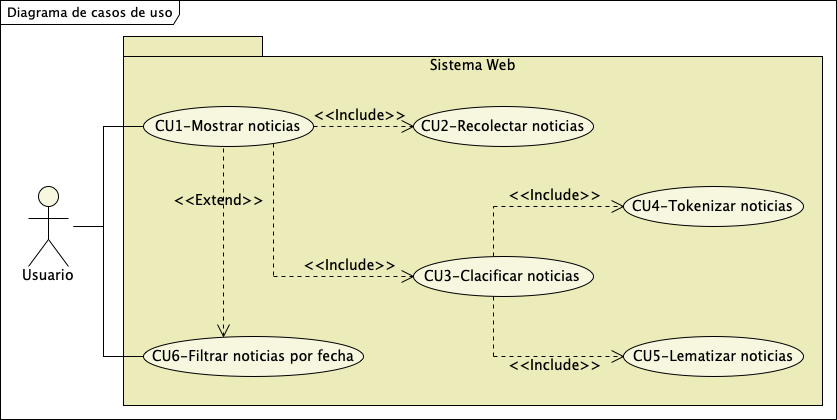
\includegraphics[scale=.4]{imagenes/Diagramas/CasosDeuso/CasosDeuso}
%  \caption{Diagrama de casos de uso}
%  \label{fig:DCU}
%\end{figure}


{\setlength{\parindent}{0pt}%Con este comando eliminos la indexación de cada párrafo%
  
  \newpage
  \input{Capitulos/Capitulo4-AnalisisYdisenio/CasosDeUso/cu1-mostrarNoticia}
  \newpage
  \input{Capitulos/Capitulo4-AnalisisYdisenio/CasosDeUso/cu2-recolectarNoticias}
  \newpage
  \input{Capitulos/Capitulo4-AnalisisYdisenio/CasosDeUso/cu3-clasificarNoticia}
  \newpage
  \input{Capitulos/Capitulo4-AnalisisYdisenio/CasosDeUso/cu4-tokenizarNoticias}
  \newpage
  \Tsubsection{CU5 Lematizar noticias}

\begin{large}
	\textbf{Resumen}\\
\end{large}

Texto.\\

\begin{large}
	\textbf{Descripción}\\
\end{large}

\begin{tabular}{|l|l|}
	\hline
	\multicolumn{1}{| >{\columncolor{black}}l|}{ \textcolor{myWhite}{\textbf{Caso de uso: }} }&
	\multicolumn{1}{| >{\columncolor{black}}l|}{ \textcolor{myWhite}{CU-1 Recolectar noticias} }\\
	\hline
	\textbf{Actor:} & 	Lorem Ipsum	\\
	\hline
	\textbf{Propósito:} & Lorem Ipsum \\
	\hline
	\textbf{Entradas:} & Lorem Ipsum \\
	\hline
	\textbf{Salidas:} & Lorem Ipsum\\
	\hline
	\textbf{Precondición:} & Lorem Ipsum \\
	\hline
	\textbf{Postcondiciones:} & Lorem Ipsum \\
	\hline
	\textbf{Reglas de negocio:} & Lorem Ipsum \\
	\hline
	\textbf{Errores:} & Lorem Ipsum \\
	\hline
	\textbf{Autor:} & Lorem Ipsum \\
	\hline
\end{tabular}\\\\

%--------------------Trayectoria Principal-----------%


\begin{large}
	\textbf{Trayectoria principal}\\
\end{large}	

\begin{enumerate}[1.]
	\item \actor lorem ipsum
	\item \sistema lorem ipsum
	\item \sistema lorem ipsum
	\item \sistema lorem ipsum
	\item \finCU	
\end{enumerate}


%--------------------trayectoria Alternatia A---------%

\begin{large}
	\textbf{Trayectoria alternativa A:}\\
\end{large}	
\textbf{Condición:} \textit{Se escribe la condición}
\begin{enumerate}[{A-}1.]

	\item \actor lorem ipsum
	\item \sistema lorem ipsum
	\item \finTA	

\end{enumerate}


%--------------------trayectoria Alternatia b---------%
\begin{large}
	\textbf{Trayectoria alternativa B:}\\
\end{large}	
\textbf{Condición:} \textit{Se escribe la condición}

\begin{enumerate}[{B-}1.]

	\item \actor lorem ipsum
	\item \sistema lorem ipsum
	\item \finTA	

\end{enumerate}


%--------------------Puntos de extención--------------------%

\begin{large}
	\textbf{Puntos de extensión}\\
\end{large}	

\textbf{Causa de la extensión:} Lorem ipsum\\
\textbf{Región de la trayectorioa:} Lorem ipsum\\
\textbf{Extiende a :} Lorem ipsum\\\\

\textbf{Causa de la extensión:} Lorem ipsum\\
\textbf{Región de la trayectorioa:} Lorem ipsum\\
\textbf{Extiende a :} Lorem ipsum\\


  \newpage
  \input{Capitulos/Capitulo4-AnalisisYdisenio/CasosDeUso/cu6-FiltrarNoticiaFecha}
  \newpage
}

%------------------------Mensajes----------------------------------%

\section{Mensajes}
  
  %------------------MSG1-----------------------%
     \Mline{MSG1}{Catálago vacio}
    \begin{itemize}
      \item \textbf{Tipo:} Error. 
      \item \textbf{Objetivo:}  Dar a conocer que no se tiene las lígas a los sitios web.
      \item \textbf{Redacción:} El catálogo \textbf{Direcciones web} se encuentra vacio.
      \item \textbf{Referenciado por:} \Tref{CU1}{CU1 Seleccionar sección}\\
    \end{itemize}

  %------------------MSG2-----------------------%
     \Mline{MSG2}{Lenguaje de sitio}
    \begin{itemize}
      \item \textbf{Tipo:} Error. 
      \item \textbf{Objetivo:}  Dar a conocer que los sitios a los cuales desea ingresar, no están redactados en lenguaje español.
      \item \textbf{Redacción:} Los sitios no se encuentran en lenguaje español, por lo cual no serán consultados.
      \item \textbf{Referenciado por:} \Tref{CU1}{CU1 Seleccionar sección}\\
    \end{itemize}

  %------------------MSG3-----------------------%
     \Mline{MSG3}{Faltan campos obligatorios}
    \begin{itemize}
      \item \textbf{Tipo:} Error. 
      \item \textbf{Objetivo:}  Dar a conocer que hay campos obligatorios vacios.
      \item \textbf{Redacción:} Los campos marcados con * no pueden omitirse.
      \item \textbf{Referenciado por:} \Tref{CU2}{CU2 Buscar noticias}\\
    \end{itemize}

  %------------------MSG4-----------------------%
   \Mline{MSG4}{Formato de feha inválido}
  \begin{itemize}
    \item \textbf{Tipo:} Error. 
    \item \textbf{Objetivo:}  Informar que se ha ingrsado una fecha no válida.
    \item \textbf{Redacción:} Se ha ingresado una fecha inválida; El formato correcto es DD/MM/AAAA.
    \item \textbf{Referenciado por:} \Tref{CU2}{CU2 Buscar noticias}\\
  \end{itemize}

    %------------------MSG5-----------------------%
   \Mline{MSG5}{Periodo no válido}
  \begin{itemize}
    \item \textbf{Tipo:} Error. 
    \item \textbf{Objetivo:}  Informar que se ha ingrsado una un perido incongruente.
    \item \textbf{Redacción:} El periodo ingresado es incorrecto.
    \item \textbf{Referenciado por:} \Tref{CU2}{CU2 Buscar noticias}\\
  \end{itemize}

    %------------------MSG6-----------------------%
   \Mline{MSG6}{Lítimes fuera de rango}
  \begin{itemize}
    \item \textbf{Tipo:} Error. 
    \item \textbf{Objetivo:}  Informar que el intervalo de tiempo está fuera de los límites del sistema.
    \item \textbf{Redacción:} El periodo ingresado está fuera de los límites permitidos, la fecha debe estar entr 01/01/1990 y el día en curso.
    \item \textbf{Referenciado por:} \Tref{CU2}{CU2 Buscar noticias}\\
  \end{itemize}

  %--------------------------Descripción de pantallas ------------------%
\section{Pantallas}

\input{Capitulos/Capitulo4-AnalisisYdisenio/DescripcionPantallas/ui1-inicio}
\newpage
\subsection{UI2-Sección deportes}

\Large{\textbf{Objetivo}}\\\\
\normalsize{Texto}\\



\Large{\textbf{Descripción}}\\
\normalsize{Texto}\\


\Large{\textbf{Comandos}}\\
\normalsize{}

\begin{itemize}
	\item Lorem ipsum
	\item Lorem ipsum
	\item Lorem ipsum
\end{itemize}

\Large{\textbf{Referencia}}\\\\
\normalsize{Nombre Caso de uso}

\begin{figure}
  \centering
	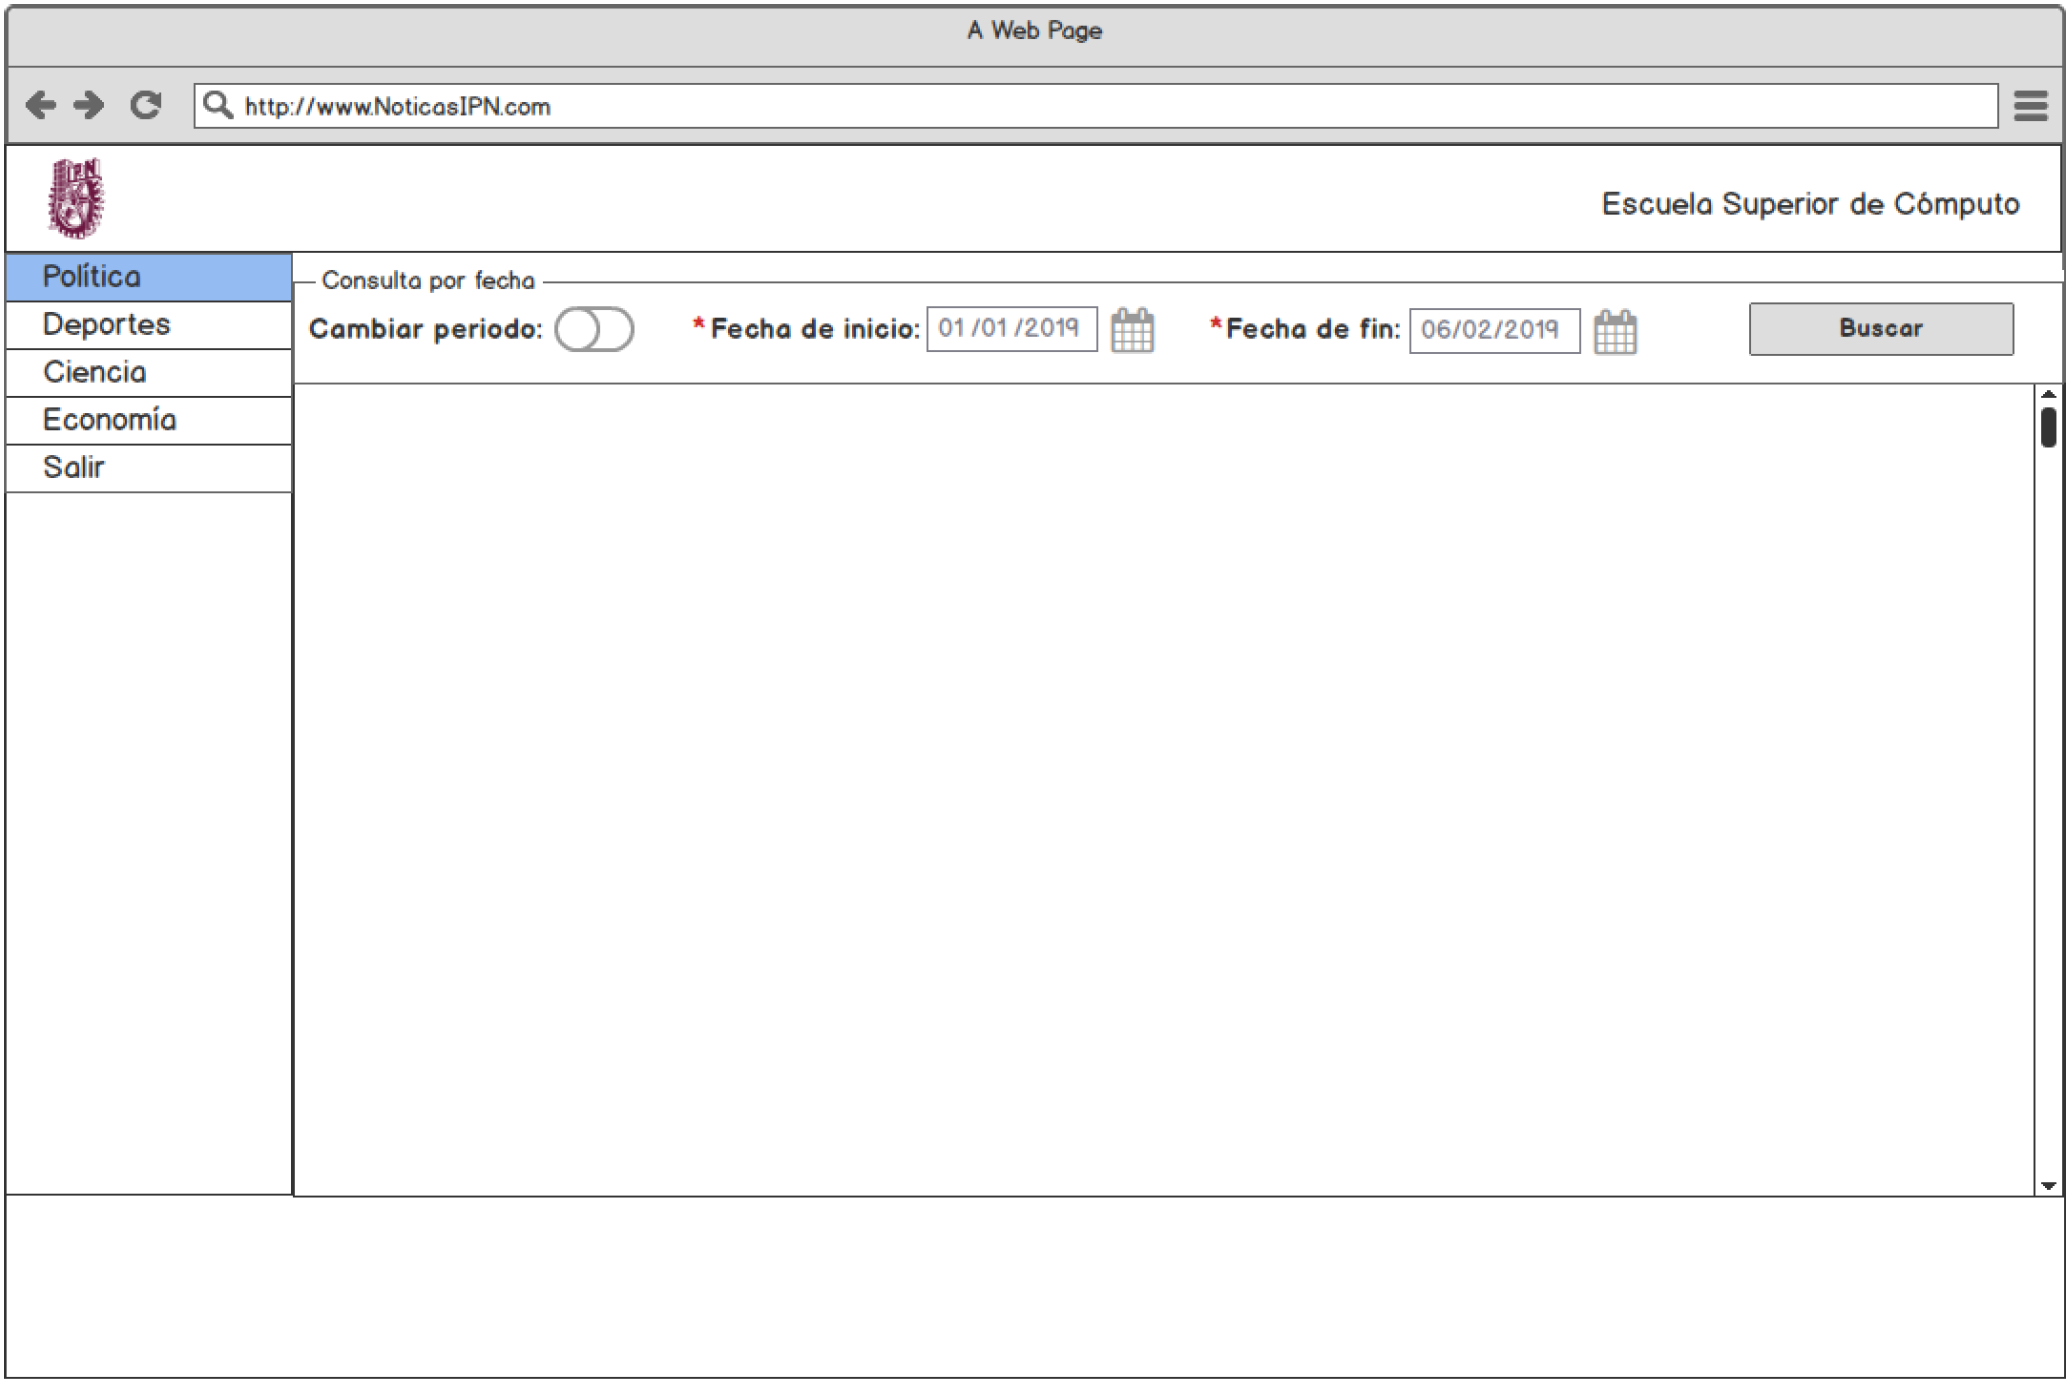
\includegraphics[scale=.3]{imagenes/Pantallas/UI2}
  \caption{Pantalla IU2-Sección deportes}
  \label{fig:IU2}
\end{figure}
\newpage
\subsection{UI3-Busqueda por fecha}

\Large{\textbf{Objetivo}}\\\\
\normalsize{Texto}\\

	

\Large{\textbf{Descripción}}\\
\normalsize{Texto}\\



\Large{\textbf{Comandos}}\\
\normalsize{}

\begin{itemize}
	\item Lorem ipsum
	\item Lorem ipsum
	\item Lorem ipsum
\end{itemize}

\Large{\textbf{Referencia}}\\\\
\normalsize{Nombre Caso de uso}

\begin{figure}[h]
  \centering
	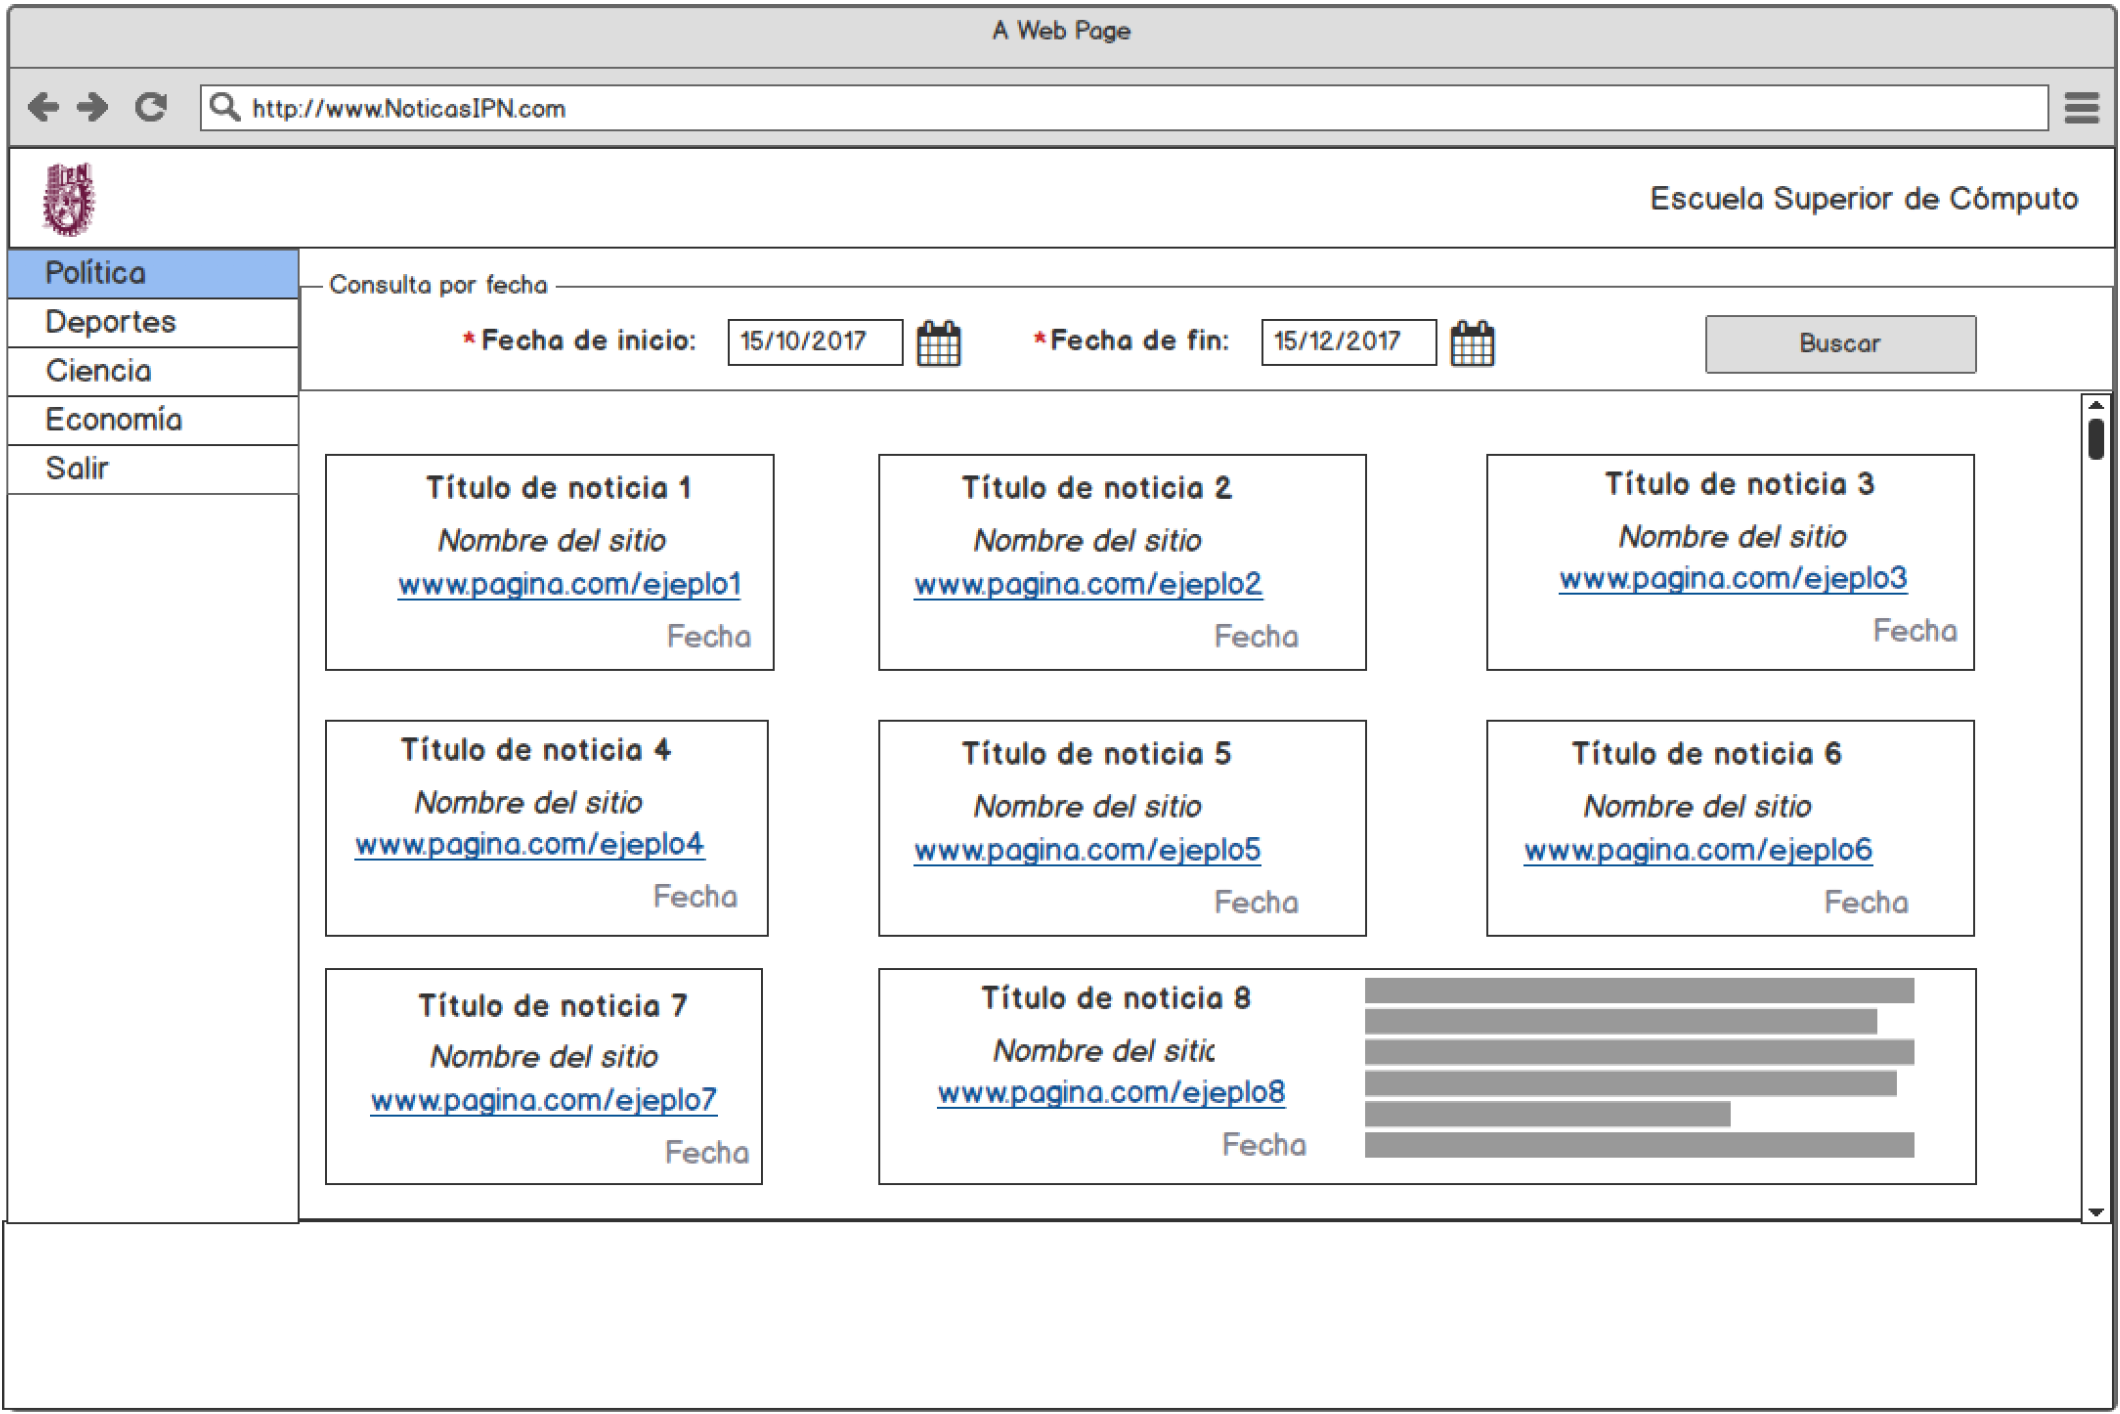
\includegraphics[scale=.3]{imagenes/Pantallas/UI3}
  \caption{Pantalla IU3-Busqueda por fecha}
  \label{fig:IU3}
\end{figure}
\newpage
\subsection{UI4-Página ejemplo}

\Large{\textbf{Objetivo}}\\\\
\normalsize{Texto}\\



\Large{\textbf{Descripción}}\\
\normalsize{Texto}\\


\Large{\textbf{Comandos}}\\
\normalsize{Texto}

\begin{itemize}
	\item Lorem ipsum
	\item Lorem ipsum
	\item Lorem ipsum
\end{itemize}

\Large{\textbf{Referencia}}\\\\
\normalsize{Nombre Caso de uso}

\begin{figure}
  \centering
	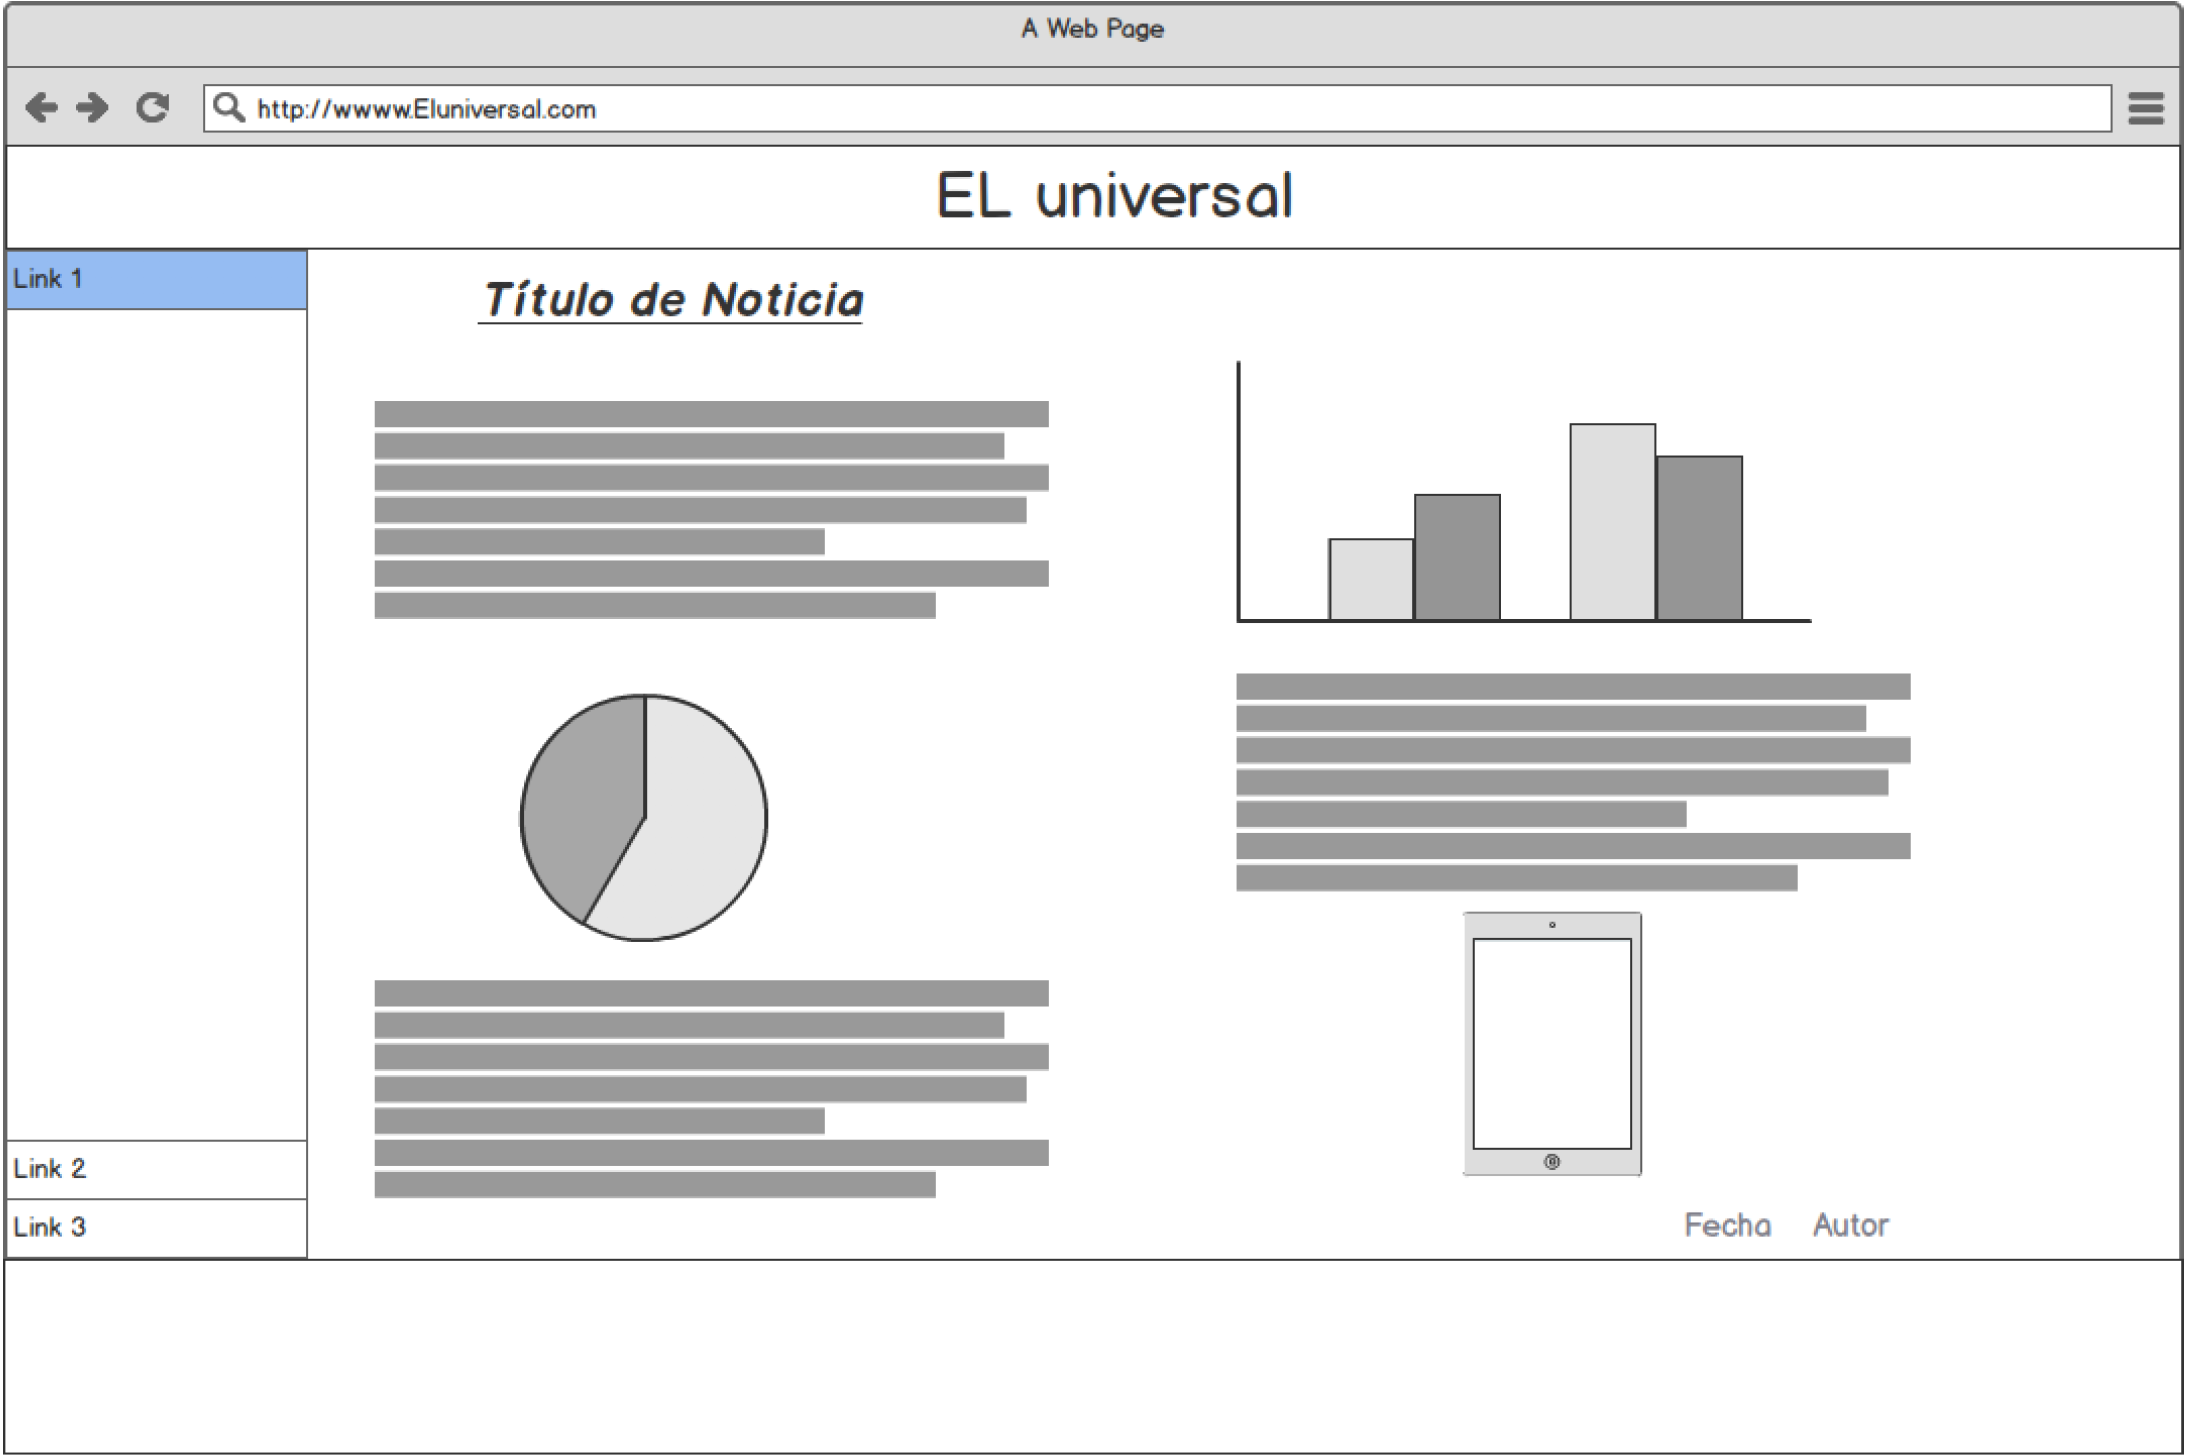
\includegraphics[scale=.3]{imagenes/Pantallas/UI4}
  \caption{Pantalla IU4-Página ejemplo}
  \label{fig:IU4}
\end{figure}
\newpage





  \newpage
   \TChapter{Avances}{epsilon}
\ \\\\
En esta sección se mostrarán los avances que hasta el día de hoy se tienen.

%-----------------------------------------------------------------------------------------%
\section{Herramientas utilizadas}
Para el desarrollo de los avances en el presente trabajo, se utilizó el lenguaje de programación Python\footnote{https://www.python.org/} 
en la distribución Anaconda\footnote{https://www.anaconda.com/distribution/}, ya que gestiona las 
versiones de las librerías utilizadas para el análisis de datos, y para el recolector web (Crawler) se utilizó Scrapy\footnote{https://scrapy.org/}, 
un framework que permite la extracción de información de sitios web.

%-----------------------------------------------------------------------------------------%

\section{Estudio previo}
Una vez elegidas las herramientas que permiten la extracción de la información, se procedió con la selección de los 
sitios web para extraer noticias.
\\
El sitio web El Economista\footnote{https://www.eleconomista.com.mx/} contiene una sección llamada 
\textbf{Ranking de Medios Nativos Digitales}\footnote{https://www.eleconomista.com.mx/Ranking-de-Medios-Nativos-Digitales}, 
el cual muestra las estadísticas que realiza mes con mes acerca de los sitios de noticias web más consultados como se muestra 
en la Figura \textbf{\ref{fig:rank}}
\begin{figure}[H]
  \centering
  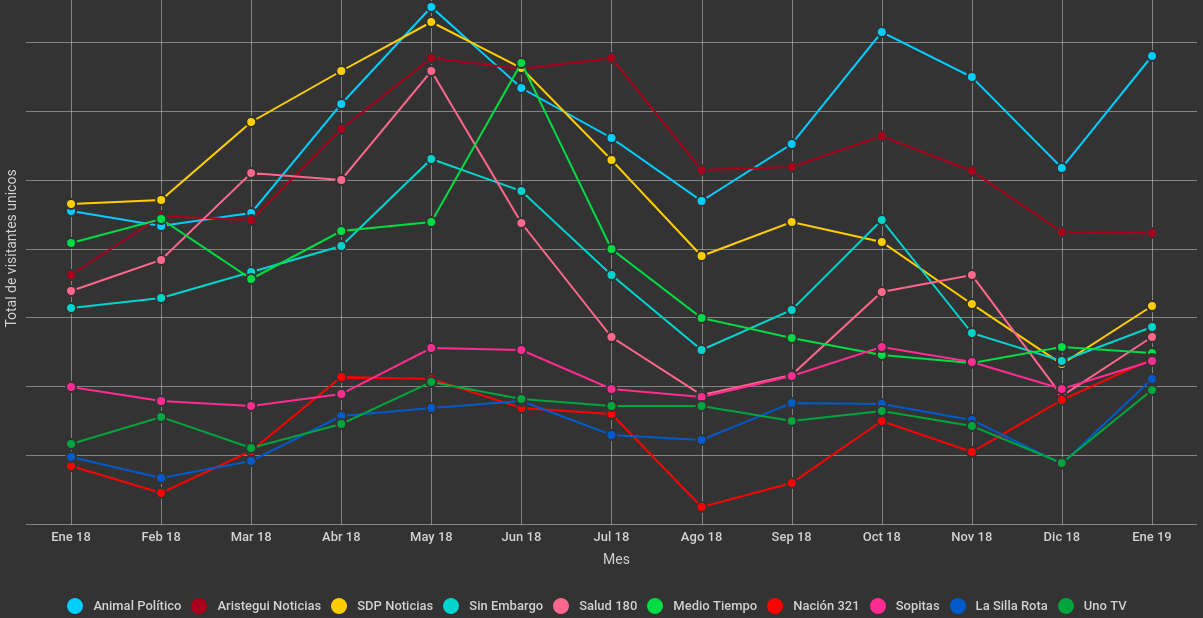
\includegraphics[scale=.28]{imagenes/Capitulo5/ranking}
  \caption{Ranking de sitios de noticias del periódo de enero del 2018 a enero del 2019.}
  \label{fig:rank}
\end{figure}
 

Para la selección final de los sitios de noticias que se utilizarán en estre trabajo, se revisaron los los medios mostrados en la Figura 5.1. Después de esta revisión se encontró que los sitios Salud 180 y Medio Tiempo muestran noticias relacionadas únicamente con salud y deportes respectivamente. En este trabajo se desean obtener noticias de diversas secciones por lo que estos sitios se descartaron. También para este trabajo es importante incluir información de otros medios como diarios y  sitios de televisón, por lo tanto se incluyeron sitios relacionados con estos medios.

\begin{itemize}
    \item 3 Sitios de foros de noticias: 
    \begin{itemize}
      \item \textbf{Aristegui Noticias}: https://aristeguinoticias.com/
      \item \textbf{SDP Noticias}: https://www.sdpnoticias.com/
      \item \textbf{Sopitas}: https://www.sopitas.com/
    \end{itemize}
    \item 3 Sitios de diarios:
    \begin{itemize}
      \item \textbf{El Universal}: https://www.eluniversal.com.mx/
      \item \textbf{La Jornada}: https://www.jornada.com.mx/
      \item \textbf{Exélsior}: https://www.excelsior.com.mx/
    \end{itemize}
    \item 3 Sitios de televisión:
    \begin{itemize}
      \item \textbf{TV Azteca}: https://www.aztecanoticias.com.mx/
      \item \textbf{Televisa}: https://noticieros.televisa.com/
      \item \textbf{Once Noticias}: https://www.oncenoticias.tv/
    \end{itemize}
\end{itemize}

Los sitios organizan las noticias en secciones. Una vez seleccionados los sitios, se procedió con el análisis de las secciones que contienen los portales, como 
lo muestra la Tabla \textbf{\ref{tabla:sitios}}.

\begin{table}[htbp]
    \centering
    \resizebox{\columnwidth}{!}{%
    \begin{tabular}[H]{|l|l|l|l|l|l|l|l|l|}


 \multicolumn{1}{| >{\columncolor{myBlueChapter}}l|}{ \textcolor{myWhite}{\textbf{El}} }
&\multicolumn{1}{| >{\columncolor{myBlueChapter}}l|}{ \textcolor{myWhite}{\textbf{La}} }
&\multicolumn{1}{| >{\columncolor{myBlueChapter}}l|}{ \textcolor{myWhite}{\textbf{Milenio}} }
&\multicolumn{1}{| >{\columncolor{myBlueChapter}}l|}{ \textcolor{myWhite}{\textbf{Aristegui}} }
&\multicolumn{1}{| >{\columncolor{myBlueChapter}}l|}{ \textcolor{myWhite}{\textbf{SDP}} }
&\multicolumn{1}{| >{\columncolor{myBlueChapter}}l|}{ \textcolor{myWhite}{\textbf{Sopitas}} }
&\multicolumn{1}{| >{\columncolor{myBlueChapter}}l|}{ \textcolor{myWhite}{\textbf{Azteca}} }
&\multicolumn{1}{| >{\columncolor{myBlueChapter}}l|}{ \textcolor{myWhite}{\textbf{Televisa}} }
&\multicolumn{1}{| >{\columncolor{myBlueChapter}}l|}{ \textcolor{myWhite}{\textbf{Once}} }
  \\ \cline{1-9}
%---------------------------------------------------------------------------------------%

 \multicolumn{1}{| >{\columncolor{myBlueChapter}}l|}{ \textcolor{myWhite}{\textbf{Universal}} }
&\multicolumn{1}{| >{\columncolor{myBlueChapter}}l|}{ \textcolor{myWhite}{\textbf{Jornada}} }
&\multicolumn{1}{| >{\columncolor{myBlueChapter}}l|}{ }
&\multicolumn{1}{| >{\columncolor{myBlueChapter}}l|}{ \textcolor{myWhite}{\textbf{Noticias}} }
&\multicolumn{1}{| >{\columncolor{myBlueChapter}}l|}{ \textcolor{myWhite}{\textbf{Noticias}} }
&\multicolumn{1}{| >{\columncolor{myBlueChapter}}l|}{ }
&\multicolumn{1}{| >{\columncolor{myBlueChapter}}l|}{ \textcolor{myWhite}{\textbf{Noticias}} }
&\multicolumn{1}{| >{\columncolor{myBlueChapter}}l|}{ }
&\multicolumn{1}{| >{\columncolor{myBlueChapter}}l|}{ \textcolor{myWhite}{\textbf{Noticias}} }
\\ \cline{1-9}

%---------------------------------------------------------------------------------------%

        Nacional      & -            & Nacional      & México                & Nacional      & Noticias  & -                 & Nacional      & Nacional      \\ 
        \hline
%---------------------------------------------------------------------------------------%

       	Mundo         & Mundo        & Mundo         & Destacado o       & Internacional & -         & Internacional     & Internacional & Internacional \\ 
        & & & Mundo & & & & & \\ 
        \hline
%---------------------------------------------------------------------------------------%

        Metrópoli     & Capital      & CDMX          & -                     & -             & -         & -                 & CDMX          & CDMX      \\ 
        \hline
%---------------------------------------------------------------------------------------%

        Estados       & Estados      & Estados       & Sociedad o       & Estados       & -         & Estados           & Estados       & Nacional   \\ 
        & & & México & & & & & \\ 
        \hline
%---------------------------------------------------------------------------------------%

        Cartera       & Economía     & Negocios      & Economía              & Economía      & -         & Finanzas          & Economía      & Economía   \\ 
        \hline
%---------------------------------------------------------------------------------------%

        Deportes      & Deportes     & La Afición    & Deportes              & Deportes      & Deportes  & -                 & Deportes      & Deportes   \\ 
        \hline
%---------------------------------------------------------------------------------------%

        Espectáculos  & Espectáculos & Hey           & -                     & En el show    & Entretenimiento & -           & Entretenimiento & Deportes    \\ 
        \hline
%---------------------------------------------------------------------------------------%

        Cultura       & Cultura      & Cultura       & -                     & -             & -         & -                 & Arte y cultura & Cultura   \\ 
        \hline
%---------------------------------------------------------------------------------------%

        Nación o & Política   & Política      & Poderes               & -             & -         & Política          & Política      & -   \\ 
        & política & & & & & & & \\ 
        \hline
%---------------------------------------------------------------------------------------%

        Ciencia y & Tecnología & Tecnología    &                       & Geek          & Geek      & -                 & Tecnología*      & Ciencia\\
        salud & & & & & & & & \\ 
        \hline        

    \end{tabular}%
}
\caption[Tabla]{Secciones existentes en los sitios web}
\label{tabla:sitios}
\end{table}

Una vez que se analizarón las secciones con las que contaba cada sitio se procedió a homologar las secciones en las cuales la mayoría de los sitios coincidian, por lo cual se quedarón definidas 5 secciones para clasificación de las noticia:

\begin{itemize}
    \item Política
    \item Deportes
    \item Ciencia y tecnología
    \item Economía
    \item Cultura
\end{itemize}

Para llevar a cabo el proceso de extracción de las noticias, se realizó el estudio 
de la estructura XML (\textit{Extensible Markup Language}), por sus siglas en inglés de cada sitio web seleccionado, con 
el objetivo de definir las etiquetas que poseen la información de las noticias, las cuales son:

\begin{itemize}
  \item URL
  \item Sección
  \item Título
  \item Autor
  \item Fecha
  \item Descripción
  \item Noticia
\end{itemize} 

%-----------------------------------------------------------------------------------------%
\section{Recolección de noticias}
En la siguiente Figura \textbf{\ref{fig:diagrama}}. se describe el proceso de recolección:

\begin{figure}[H]
  \centering
  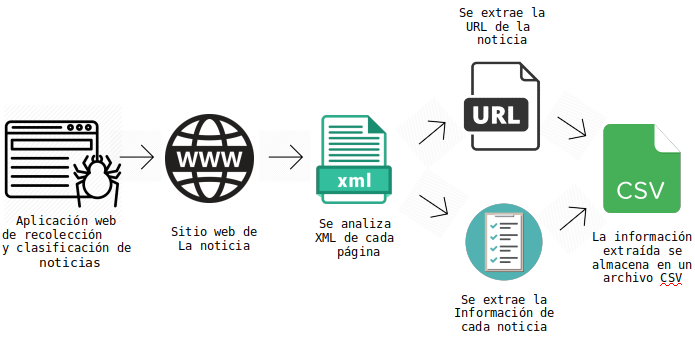
\includegraphics[scale=.50]{imagenes/Capitulo5/diagrama}
  \caption{Proceso de recolección de noticias.}
  \label{fig:diagrama}
\end{figure}

%-----------------------------------------------------------------------------------------%
\subsection{Desarrollo}

Con base en la información obtenida de los sitios web, se diseño un recolector de noticias para cada sitio, procede con 
los siguientes pasos para realizar la extracción de noticias.

\begin{itemize}
  \item Se ingresa a la URL definida como inicio y se analiza la etiqueta definida que redirecciona a cada noticia del sitio web
  \item Una vez que se ha ingresado a la noticia se procede con el análisis de las etiquetas definidas
  \item Se extrae la información de cada noticia, así como su URL
  \item Posteriormente la información recolectada se guarda en un archivo csv
\end{itemize}
La siguiente figura muestra el comando que realiza el proceso de recolección de las noticias.

%Para el proceso de extracción se abre una terminal con la ruta donde se guardará la información recolectada Figura \textbf{\ref{fig:uno}} 
%Se va a redactar los pasos del proceso de recolección

%-----------------------------------------------------------------------------------------%
\subsection{Resultados}

%-----------------------------------------------------------------------------------------%
\subsubsection{Secciones recolectadas}

De los nueve sitios web definidos se obtuvieros las siguientes secciones mostrados en la Tabla \textbf{\ref{tabla:secciones}}:
\\
\begin{table}[htbp]
  \centering
  \resizebox{\columnwidth}{!}{%
  \begin{tabular}{|c|c|c|c|c|c|c|c|c|c|}

 \multicolumn{1}{| >{\columncolor{myBlueChapter}}l|}{ \textcolor{myWhite}{\textbf{Sección}} }
&\multicolumn{1}{| >{\columncolor{myBlueChapter}}l|}{ \textcolor{myWhite}{\textbf{El}} }
&\multicolumn{1}{| >{\columncolor{myBlueChapter}}l|}{ \textcolor{myWhite}{\textbf{La}} }
&\multicolumn{1}{| >{\columncolor{myBlueChapter}}l|}{ \textcolor{myWhite}{\textbf{Milenio}} }
&\multicolumn{1}{| >{\columncolor{myBlueChapter}}l|}{ \textcolor{myWhite}{\textbf{Aristegui}} }
&\multicolumn{1}{| >{\columncolor{myBlueChapter}}l|}{ \textcolor{myWhite}{\textbf{SDP}} }
&\multicolumn{1}{| >{\columncolor{myBlueChapter}}l|}{ \textcolor{myWhite}{\textbf{Sopitas}} }
&\multicolumn{1}{| >{\columncolor{myBlueChapter}}l|}{ \textcolor{myWhite}{\textbf{Azteca}} }
&\multicolumn{1}{| >{\columncolor{myBlueChapter}}l|}{ \textcolor{myWhite}{\textbf{Televisa}} }
&\multicolumn{1}{| >{\columncolor{myBlueChapter}}l|}{ \textcolor{myWhite}{\textbf{Once}} }
  \\ \cline{1-10}
%---------------------------------------------------------------------------------------%
 \multicolumn{1}{| >{\columncolor{myBlueChapter}}l|}{ }
&\multicolumn{1}{| >{\columncolor{myBlueChapter}}l|}{ \textcolor{myWhite}{\textbf{Universal}} }
&\multicolumn{1}{| >{\columncolor{myBlueChapter}}l|}{ \textcolor{myWhite}{\textbf{Jornada}} }
&\multicolumn{1}{| >{\columncolor{myBlueChapter}}l|}{ }
&\multicolumn{1}{| >{\columncolor{myBlueChapter}}l|}{ \textcolor{myWhite}{\textbf{Noticias}} }
&\multicolumn{1}{| >{\columncolor{myBlueChapter}}l|}{ \textcolor{myWhite}{\textbf{Noticias}} }
&\multicolumn{1}{| >{\columncolor{myBlueChapter}}l|}{ }
&\multicolumn{1}{| >{\columncolor{myBlueChapter}}l|}{ \textcolor{myWhite}{\textbf{Noticias}} }
&\multicolumn{1}{| >{\columncolor{myBlueChapter}}l|}{ }
&\multicolumn{1}{| >{\columncolor{myBlueChapter}}l|}{ \textcolor{myWhite}{\textbf{Noticias}} }
\\ \cline{1-10}


  %---------------------------------Economía--------------------------------------%  
  Economía & \Checkmark & \Checkmark & \Checkmark & \Checkmark & \Checkmark & \XSolidBrush & \Checkmark & \Checkmark & \Checkmark \\
  \hline
  %-----------------------------------Deportes------------------------------------%  

  Deportes & \Checkmark & \Checkmark & \Checkmark & \Checkmark & \Checkmark & \Checkmark & \XSolidBrush & \Checkmark & \Checkmark \\
  \hline

  %-----------------------------------Cultura------------------------------------%  
  Cultura & \Checkmark & \Checkmark & \Checkmark & \XSolidBrush & \XSolidBrush & \XSolidBrush & \XSolidBrush & \Checkmark & \Checkmark \\
  \hline

  %-----------------------------------Política------------------------------------%  
  Política  & \Checkmark & \Checkmark & \Checkmark & \Checkmark & \XSolidBrush & \XSolidBrush & \Checkmark & \Checkmark & \XSolidBrush \\
  \hline

  %-------------------------------Ciencia y tecnología-----------------------------------%  
  Ciencia y& \Checkmark & \Checkmark & \Checkmark & \XSolidBrush & \Checkmark & \Checkmark & \XSolidBrush & \Checkmark & \Checkmark \\
  tecnología  & & & & & & & & & \\
  \hline

    \end{tabular}%
}
\caption{Secciones contenidas en los sitios web definidos}
\label{tabla:secciones}
\end{table}

%-----------------------------------------------------------------------------------------%
\subsubsection{Resultados de las etiquetas}
En la Tabla \textbf{\ref{tabla:etiquetas}}, muestra los campos que pueden ser extraídos por cada sitio.
%Expresar la idea de que se intento recolectar toda la información sin embargo no se pueo 
\begin{table}[htbp]
  \centering
  \resizebox{\columnwidth}{!}{%
  \begin{tabular}{|c|c|c|c|c|c|c|c|c|c|}

 \multicolumn{1}{| >{\columncolor{myBlueChapter}}l|}{ \textcolor{myWhite}{\textbf{Etiqueta}} }
&\multicolumn{1}{| >{\columncolor{myBlueChapter}}l|}{ \textcolor{myWhite}{\textbf{El}} }
&\multicolumn{1}{| >{\columncolor{myBlueChapter}}l|}{ \textcolor{myWhite}{\textbf{La}} }
&\multicolumn{1}{| >{\columncolor{myBlueChapter}}l|}{ \textcolor{myWhite}{\textbf{Milenio}} }
&\multicolumn{1}{| >{\columncolor{myBlueChapter}}l|}{ \textcolor{myWhite}{\textbf{Aristegui}} }
&\multicolumn{1}{| >{\columncolor{myBlueChapter}}l|}{ \textcolor{myWhite}{\textbf{SDP}} }
&\multicolumn{1}{| >{\columncolor{myBlueChapter}}l|}{ \textcolor{myWhite}{\textbf{Sopitas}} }
&\multicolumn{1}{| >{\columncolor{myBlueChapter}}l|}{ \textcolor{myWhite}{\textbf{Azteca}} }
&\multicolumn{1}{| >{\columncolor{myBlueChapter}}l|}{ \textcolor{myWhite}{\textbf{Televisa}} }
&\multicolumn{1}{| >{\columncolor{myBlueChapter}}l|}{ \textcolor{myWhite}{\textbf{Once}} }
  \\ \cline{1-10}
%---------------------------------------------------------------------------------------%
 \multicolumn{1}{| >{\columncolor{myBlueChapter}}l|}{ }
&\multicolumn{1}{| >{\columncolor{myBlueChapter}}l|}{ \textcolor{myWhite}{\textbf{Universal}} }
&\multicolumn{1}{| >{\columncolor{myBlueChapter}}l|}{ \textcolor{myWhite}{\textbf{Jornada}} }
&\multicolumn{1}{| >{\columncolor{myBlueChapter}}l|}{ }
&\multicolumn{1}{| >{\columncolor{myBlueChapter}}l|}{ \textcolor{myWhite}{\textbf{Noticias}} }
&\multicolumn{1}{| >{\columncolor{myBlueChapter}}l|}{ \textcolor{myWhite}{\textbf{Noticias}} }
&\multicolumn{1}{| >{\columncolor{myBlueChapter}}l|}{ }
&\multicolumn{1}{| >{\columncolor{myBlueChapter}}l|}{ \textcolor{myWhite}{\textbf{Noticias}} }
&\multicolumn{1}{| >{\columncolor{myBlueChapter}}l|}{ }
&\multicolumn{1}{| >{\columncolor{myBlueChapter}}l|}{ \textcolor{myWhite}{\textbf{Noticias}} }
\\ \cline{1-10}

  %-----------------------------------URL------------------------------------%  
      URL         & \Checkmark & \Checkmark & \Checkmark & \Checkmark & \Checkmark & \Checkmark & \Checkmark & \Checkmark & \Checkmark \\
      \hline

  %-----------------------------------Sección------------------------------------%  
      Sección     & \Checkmark & \Checkmark & \Checkmark & \Checkmark & \Checkmark & \Checkmark & \Checkmark & \Checkmark & \Checkmark \\ 
      \hline

  %-----------------------------------Título------------------------------------%  
      Título      & \Checkmark & \Checkmark & \Checkmark & \Checkmark & \Checkmark & \Checkmark & \Checkmark & \Checkmark & \Checkmark \\ 
      \hline

  %----------------------------------Autor-----------------------------------%  
      Autor       & \Checkmark & \Checkmark & \Checkmark & \Checkmark & \Checkmark & \Checkmark & \Checkmark & \Checkmark & \Checkmark \\ 
      \hline
  %------------------------------------Fecha--------------------------------------%  
      Fecha       & \Checkmark & \Checkmark & \Checkmark & \Checkmark & \Checkmark & \Checkmark & \Checkmark & \Checkmark & \Checkmark \\ 
      \hline
  %-----------------------------------Descripción------------------------------------%  
      Descripción & \Checkmark & \XSolidBrush & \Checkmark & \XSolidBrush & \XSolidBrush & \Checkmark & \Checkmark & \Checkmark & \Checkmark \\ 
      \hline
  %-----------------------------------Noticia------------------------------------%  
      Noticia     & \Checkmark & \Checkmark & \Checkmark & \Checkmark & \Checkmark & \Checkmark & \Checkmark & \Checkmark & \Checkmark \\ 
      \hline

    \end{tabular}%
}
\caption{Etiquetas extraídos de cada sitio web}
\label{tabla:etiquetas}
\end{table}

%-----------------------------------------------------------------------------------------%
\subsubsection{Archivo obtenido}

De cada sitio web se extrajeron los artículos y URLs (noticias asociadas) contenidos en la página principal, 
almacenados en un archivo CSV\footnote{Un documento CSV es un archivo de formato simple utilizado para almacenar información tabular} como se muestra 
en la Figura \textbf{\ref{fig:nueve}}. Cabe destacar que posteriormente la información recolectada será utilizada 
como parte del corpus de entrenamiento del clasificador.

\begin{figure}[H]
  \centering
  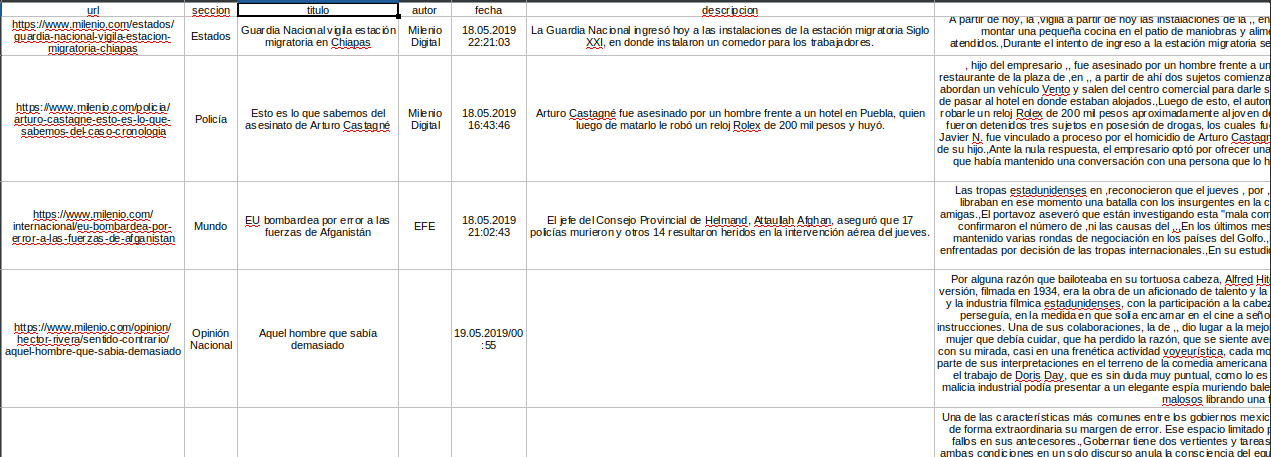
\includegraphics[scale=.3]{imagenes/Capitulo5/9}
  \caption{Resultados obtenidos de la extracción del sitio web almacenado en un archivo CSV.}
  \label{fig:nueve}
\end{figure}

%-----------------------------------------------------------------------------------------%
\subsection{Consideraciones}
\begin{itemize}
  \item Se debe tener conocimiento de XML para poder realizar las etiquetas que extraen información de la cada sitio web
  \item Cuando la noticia consta de un video, no se obtiene ninguna información adicional de la noticia
  \item Se debe tomar en cuenta que las secciones no están homologadas, es decir a pesar de que de la misma página existan varias secciones 
en la cual una noticia puede ser clasificada.
  \item La distribución de la información de una noticia varia dependiendo a la sección y sitio web.
  \item Se acotó el periodo de búsqueda de noticias ya que algunos sitios web muestran las noticias más recientes.
\end{itemize}

%-----------------------------------------------------------------------------------------%
\subsection{Conclusiones}
%Conclusiones
%A pesar de extraer la mayoría de etiquetas requeridas, existen algunos datos que se encuentran en una sola etiqueta.
El 75\% de los sitios web seleccionados contienen las secciones definidas. sin embargo
los sitios web de foros de noticias (Aristegui Noticias, SDP Noticias y Sopitas) tienen muy pocas secciones. A demás 
se logró desarrollar un recolector de noticias que permite extraer el contenido deseado de cada portal como las secciones de los artículos y las URLs que dirigen a noticias asociadas.

%Escribirlo de manera más precisa

%-----------------------------------------------------------------------------------------%
\section{Trabajo a futuro}
\begin{itemize}
  \item Una vez que se obtuvo la extracción de las noticias, analizarán para su integración al corpus
  \item Corregir las reglas para la extracción de la información de los sitios web, y así evitar extraer información con código HTML
  \item Agregar reglas para cada etiqueta, de manera tal manera que se obtenga la información necesaria
  \item Realizar el clasificador de noticias aplicando las técnicas de clasificación previamente definidas
\end{itemize}



  
  %-------------------------------Bibliografía----------%
  \bibliography{Capitulos/Referencia}


\end{document}
